%% LyX 2.3.7 created this file.  For more info, see http://www.lyx.org/.
%% Do not edit unless you really know what you are doing.
\documentclass[10pt,twoside,twocolumn,british,english,UKenglish]{article}
\usepackage{mathptmx}
\usepackage{berasans}
\usepackage[T1]{fontenc}
\usepackage[latin9]{inputenc}
\usepackage[letterpaper]{geometry}
\geometry{verbose,tmargin=3cm,bmargin=3cm,lmargin=1.5cm,rmargin=1.5cm,footskip=2cm,columnsep=1cm}
\usepackage{fancyhdr}
\pagestyle{fancy}
\setcounter{secnumdepth}{5}
\setcounter{tocdepth}{5}
\setlength{\parskip}{\medskipamount}
\setlength{\parindent}{0pt}
\usepackage{array}
\usepackage{refstyle}
\usepackage{textcomp}
\usepackage{amsmath}
\usepackage{amsthm}
\usepackage{graphicx}
\usepackage{rotfloat}
\usepackage{nameref}

\makeatletter

%%%%%%%%%%%%%%%%%%%%%%%%%%%%%% LyX specific LaTeX commands.

\AtBeginDocument{\providecommand\secref[1]{\ref{sec:#1}}}
\AtBeginDocument{\providecommand\tabref[1]{\ref{tab:#1}}}
\AtBeginDocument{\providecommand\parref[1]{\ref{par:#1}}}
\AtBeginDocument{\providecommand\subsecref[1]{\ref{subsec:#1}}}
\newcommand{\noun}[1]{\textsc{#1}}
%% Because html converters don't know tabularnewline
\providecommand{\tabularnewline}{\\}
\RS@ifundefined{subsecref}
  {\newref{subsec}{name = \RSsectxt}}
  {}
\RS@ifundefined{thmref}
  {\def\RSthmtxt{theorem~}\newref{thm}{name = \RSthmtxt}}
  {}
\RS@ifundefined{lemref}
  {\def\RSlemtxt{lemma~}\newref{lem}{name = \RSlemtxt}}
  {}


%%%%%%%%%%%%%%%%%%%%%%%%%%%%%% Textclass specific LaTeX commands.
\numberwithin{equation}{section}
\numberwithin{figure}{section}
\numberwithin{table}{section}

\@ifundefined{date}{}{\date{}}
%%%%%%%%%%%%%%%%%%%%%%%%%%%%%% User specified LaTeX commands.
\usepackage{draftwatermark}
\SetWatermarkText{\textsc{Prototype}}
% \SetWatermarkColor[rgb]{0.8,0.9,0.8}
\SetWatermarkFontSize{1cm}
\SetWatermarkScale{5}

\usepackage[missing=Help!,notags={No tags?},dirty=dirty]{gitinfo2}

\PassOptionsToPackage{UKenglish}{babel}
\usepackage[UKenglish]{babel}% http://ctan.org/pkg/babel
\usepackage{fancyhdr}
\usepackage[UKenglish]{datetime}
\usepackage{lastpage}
\usepackage{lipsum}

\usepackage{hyperref}
\hypersetup{
plainpages    = true,
         breaklinks    = true,% not default in dvips mode, so we must specify
         hypertexnames = false,%not ideal, but needed when pagenums duplicate (`i' vs. `1')
         pageanchor    = true,
         anchorcolor   = blue,
         colorlinks    = true, %Colours links instead of ugly boxes
         urlcolor      = blue, %Colour for external hyperlinks
         linkcolor     = blue, %Colour of internal links
         citecolor     = red %Colour of citations
}

\fancyhf{}

\renewcommand{\headrulewidth}{1pt}
\renewcommand{\footrulewidth}{1pt}

\fancyhead[C]{1839 English Rules}
\fancyhead[LE,RO]{\textit{ \nouppercase{\leftmark}} }
\fancyhead[LO,RE]{\textit{ \nouppercase{\rightmark}} }

\fancyfoot[LE,RO]{ Version: \gitFirstTagDescribe}
\fancyfoot[LO,RE]{ Date: \gitCommitterDate}

\fancyfoot[C]{Page: \thepage\  of  \pageref{LastPage}}

\pagestyle{fancy}

% https://tex.stackexchange.com/questions/121865/nameref-how-to-display-section-name-and-its-number
\newcommand*{\fullref}[1]{\hyperref[{#1}]{\autoref*{#1} \nameref*{#1}}} % One single link
\let\ref\fullref

\makeatother

\usepackage{babel}
\begin{document}
\author{\noun{English Rules}\\
\noun{Game design: J C Lawrence}}
\title{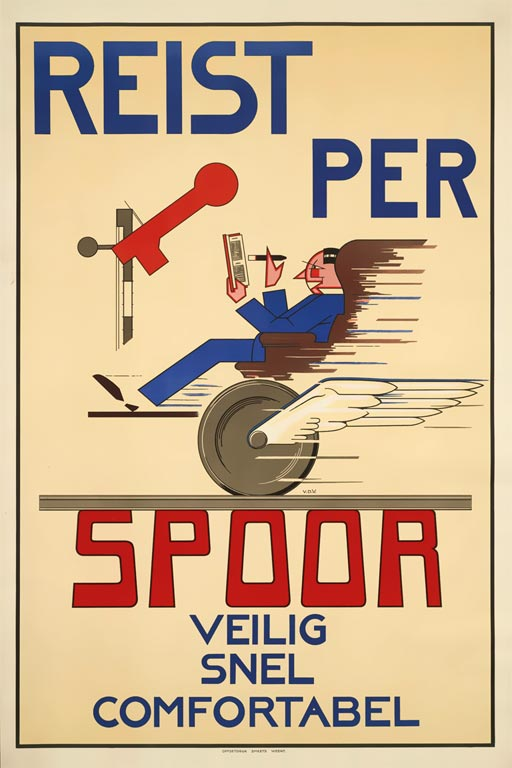
\includegraphics[height=7in]{masthead}}

\maketitle
\tableofcontents{}

\clearpage{}

\part{Overview\label{par:Overview}}

\section{Introduction\label{sec:Introduction}}

On 20 September 1839 the locomotive \noun{De Arend} made the 16 kilometer
journey between \noun{Amsterdam} and \noun{Haarlem}. After that, it
was difficult.

\begin{figure}
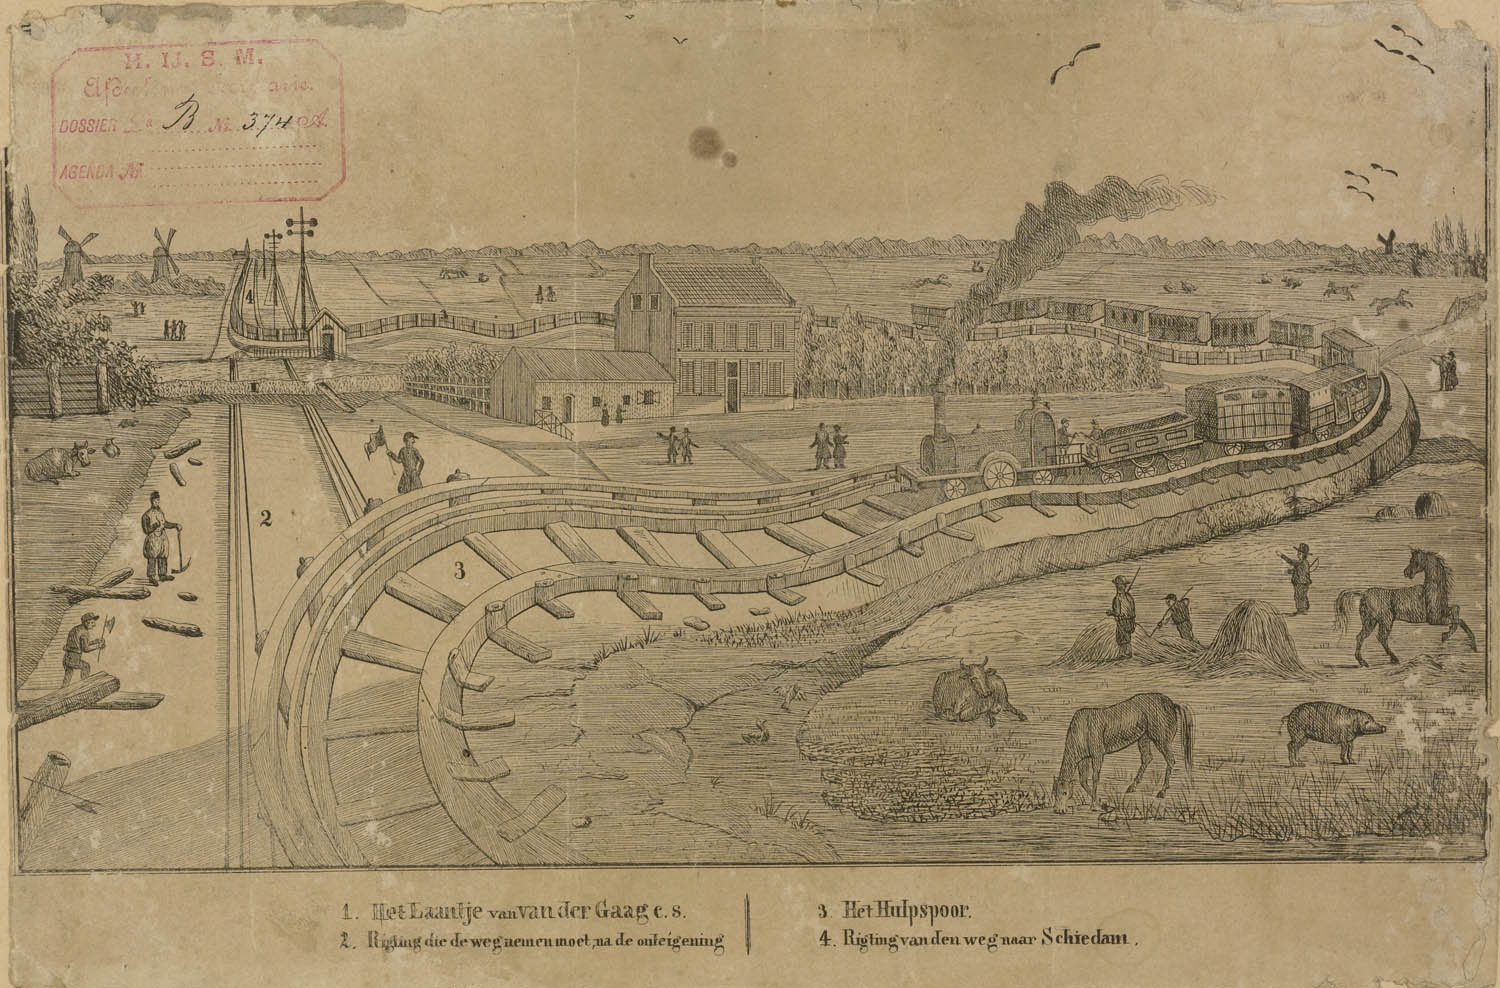
\includegraphics[width=3.5in]{laantja-vander-gaag}

\caption{The \noun{Hollandsche IJzeren Spoorweg-Maatschappij} was forced to
build a round-about loop when Aernout Hendrik van Wickevoort Crommelin's
farm refused to allow the railway to cross his property. This was
then the subject of humorous songs, postcards, comedic skits and plays
etc across Europe. Traces of the looping diversion remain visible
on satellite photographs to this day. }
\end{figure}

The player with the largest net worth at the end of the game wins
(see \secref{Game-End} \nameref{sec:Game-End}).
\begin{itemize}
\item 1 set of game rules (this document).
\item 1 game map.
\item 1 stock market (also contains the round track).
\item 1 Private auction sheet.
\item Many track tiles (yellow, green, brown and gray).
\item Trains (see \tabref{Game-Phases} \nameref{tab:Game-Phases}).
\item 2 sets of player number cards numbered 1 through 4 (one set blue \&
one set red).
\item For each of 16 Public Companies:
\begin{itemize}
\item Public company charter.
\item 9 share certificates:
\begin{itemize}
\item One 20\% director's share certificate.
\item Eight 10\% share certificates.
\end{itemize}
\item 3, 4 or 5 station markers (varies by company, see \tabref{Public-Companies}
\nameref{tab:Public-Companies}).
\item 1 stock price marker
\end{itemize}
\item 13 private companies (2 yellow, 2 green, 5 blue, 3 brown, 1 red).
\item 1 charter to track the \noun{Koninklijke Fabriek van Stoom en andere
Werktuigen}'s blue private company's revenue (see \parref{Koninklijke-Nederlandsche-Fabriek}
\nameref{par:Koninklijke-Nederlandsche-Fabriek}).
\item 32 government station markers \emph{(not count-limited)}.
\item 1 round marker.
\item \textasciitilde\foreignlanguage{british}{\textflorin }30,000 in
money \emph{(not provided)}.
\end{itemize}

\section{Etiquette\label{sec:Etiquette}}
\begin{itemize}
\item To help the game progress smoothly, each player should consider their
upcoming choices while other players are taking their turns.
\item Use of paper, pencils/pens, calculators and similar aids is recommended
to assist players in making timely and accurate decisions.
\item Players should act simultaneously when doing so would not otherwise
affect the game, such as when operating Public Companies whose choices
do not affect each other.
\end{itemize}

\part{Rules\label{part:Rules}}

\section{Setup\label{sec:Game-Setup}}
\begin{itemize}
\item Place the map, stock market, Public Company charters, shares and track
tiles where they can be easily seen and accessed.
\item Place the money nearby as the bank.
\item Pick otherwise unused areas around the board to serve as the IPO and
Bank Pool\emph{.}
\item Place the round marker on the ``SR'' space on the round track on
the Stock Market.
\item (\emph{2-player games only}) Discard the following from the game:
\begin{itemize}
\item \#3 and \#4 player number cards of both colours.
\item Private companies: 
\begin{itemize}
\item Blue: \noun{Koninklijke Fabriek van Stoom en andere Werktuigen} \&
\noun{Cr�dit Mobilier}
\item Red: \noun{Rotterdamsche Handelsvereeniging}
\end{itemize}
\end{itemize}
\begin{description}
\item [{\emph{Note:}}] \emph{The designer recommends the players in a 2-player
game already be very familiar and comfortable with 1839.}
\end{description}
\item (\emph{3-player games} \emph{only}) Discard the following from the
game:
\begin{itemize}
\item \#4 player number cards of both colours.
\item Private companies: 
\begin{itemize}
\item Blue: \noun{Cr�dit Mobilier}
\item Red: \noun{Rotterdamsche Handelsvereeniging}
\end{itemize}
\end{itemize}
\item Place the remaining private companies where they can be easily examined
by all players.
\item Take a dark brown R4 train from the supply and place it with the \noun{Diepenbrock
en Reigers te Ulft }blue private company (see \ref{par:Diepenbrock-en-Reigers})
\item Randomly assign a 20\% director's share certificate of a Spoorwegmaatschappij
(see \tabref{Public-Companies} \nameref{tab:Public-Companies} \&
\subsecref{Public-Company-Overview} \nameref{subsec:Public-Company-Overview})
and a matching 10\% share certificate to each of the three brown private
companies.
\begin{description}
\item [{Note:}] \emph{In games with players new to 1839 it is recommended
that the AMS, NBDS and ZHESM not be assigned to the }\noun{Albert
Voombergh}\emph{ brown private company (see \parref{Brown-private-companies}\nameref{par:Brown-private-companies}).}
\end{description}
\item Assign two 10\% share certificates of the Public Company assigned
to the \noun{Albert Voombergh} brown private company to the \noun{Weefgoederenfabrique
C.T. Stork \& Co} blue private company.
\item Assign the 20\% director's share certificate of a Lokaalspoorwegen
and two matching 10\% share certificates to each of the two yellow
private companies (see \tabref{Public-Companies} \nameref{tab:Public-Companies}
\& \subsecref{Public-Company-Overview} \nameref{subsec:Public-Company-Overview}). 
\item Assign one 10\% share certificate of the Public Company assigned to
the \noun{August Borsig} brown private company to the \noun{J J Beijnes}
yellow private company.
\item Separate the player number cards by colour, set one colour aside and
randomly assign the remaining player number cards, one card per player.
\item Give each player \foreignlanguage{british}{money from the bank:}
\begin{itemize}
\item 2-players: \textflorin 700
\item 3-players: \textflorin 500
\item 4-players: \textflorin 420
\end{itemize}
\end{itemize}
\begin{sidewaystable*}
\begin{description}
\item [{%
\begin{tabular}{>{\centering}m{0.6in}>{\centering}m{2cm}>{\centering}m{1in}>{\centering}m{0.6in}>{\centering}m{0.6in}>{\centering}m{0.5in}>{\centering}m{0.8in}>{\centering}m{0.8in}>{\centering}m{0.8in}>{\centering}m{0.8in}}
Phase & \multicolumn{5}{c}{Train} & Track\\
 Tiles & Operating Rounds\\
 per Set & \multicolumn{2}{c}{Available Pars}\tabularnewline
\cline{2-6} \cline{3-6} \cline{4-6} \cline{5-6} \cline{6-6} \cline{9-10} \cline{10-10} 
 & Type & Quantity & Cost & Rusts & Limit &  &  & Local & Major\tabularnewline
\hline 
Light Yellow & 2 & 5 & \textflorin 80 &  & 3 & Yellow & 1 & \textflorin 20, \textflorin 31,\\
 \textflorin 46 & \textflorin 67, \textflorin 74\\
 \& \textflorin 82\tabularnewline
\hline 
Dark Yellow & 2+1 & 4 & \textflorin 120 &  & 3 & Yellow & 1 & \textflorin 20, \textflorin 31,\\
 \textflorin 46 & \textflorin 67, \textflorin 74\\
 \& \textflorin 82\tabularnewline
\hline 
Light Green & 3 & 5  & \textflorin 140 &  & 3 & Yellow\\
Green & 2 & \textflorin 20, \textflorin 31,\\
 \textflorin 46 & \textflorin 67, \textflorin 74\\
 \& \textflorin 82\tabularnewline
\hline 
Dark Green & 3+ & 3  & \textflorin 180 & Light Yellow & 3 & Yellow\\
Green & 2 & \textflorin 20, \textflorin 31,\\
 \textflorin 46 & \textflorin 67, \textflorin 74\\
 \& \textflorin 82\tabularnewline
\hline 
Blue & 5+ & 4 & \textflorin 240 & Dark Yellow & 3 & Yellow\\
Green & 2 & \textflorin 20, \textflorin 31,\\
 \textflorin 46 & \textflorin 67 \& \textflorin 74\tabularnewline
\hline 
Light Brown & R5 & 4 & \textflorin 320 & Light Green & 3 & Yellow\\
Green\\
Brown & 2 & \textflorin 20, \textflorin 31,\\
 \textflorin 46 & \textflorin 67\tabularnewline
\hline 
Medium Brown & R4+1 & 2 & \textflorin 340 & Dark Green & 3 & Yellow\\
Green\\
Brown & 2 & \textflorin 20, \textflorin 31,\\
 \textflorin 46 & \textflorin 67\tabularnewline
\hline 
Dark Brown & R4 & 3 & \textflorin 380 & Blue &  & Yellow\\
Green\\
Brown & 2 & \textflorin 20, \textflorin 31,\\
 \textflorin 46 & \textflorin 67\tabularnewline
\hline 
Light Red & PR2+ & 4 & \textflorin 240 & Light Brown & 3 & Yellow\\
Green\\
Brown & 3 & \textflorin 20, \textflorin 31,\\
 \textflorin 46 & \textflorin 67\tabularnewline
\hline 
Dark Red & PR3+1 & 2 & \textflorin 260 & Medium Brown & 2 & Yellow\\
Green\\
Brown & 3 & \textflorin 20, \textflorin 31,\\
 \textflorin 46 & \textflorin 67\tabularnewline
\hline 
Gray & 4 & 4 & \textflorin 460 & Dark Brown & 2 & Yellow\\
Green\\
Brown\\
Gray & 3 & \textflorin 20, \textflorin 31,\\
 \textflorin 46 & \textflorin 67\tabularnewline
\hline 
Purple & 7 & Unlimited\\
(10 supplied) & \textflorin 640 & Light Red\\
\&\\
Dark Red & 2 & Yellow\\
Green\\
Brown\\
Gray & 3 & \textflorin 20, \textflorin 31,\\
 \textflorin 46 & \textflorin 67\tabularnewline
\hline 
\end{tabular}}]~
\end{description}
\centering{}\caption{Game Phases\label{tab:Game-Phases}}
\end{sidewaystable*}


\section{Game Overview \label{sec:game-overview}}
\begin{itemize}
\item 1839 begins with the auction of the private companies (see \secref{Private-Auction}
\nameref{sec:Private-Auction}).
\item After auctioning the private companies, the game consists of an alternating
series of Stock Rounds and sets of one to three Operating Rounds\noun{.
}The round marker is used to track the game's progress through the
rounds.
\item In Stock Rounds, players may buy and sell shares of Public Companies,
take and lose directorship of Public Companies (see \secref{Companies}
\nameref{sec:Companies}) and float new Public Companies (see \secref{Stock-Rounds}
\nameref{sec:Stock-Rounds}). 
\begin{itemize}
\item At the end of each Stock Round, the player order for the next Stock
Round is determined by the order in which the players cease acting
(see \subsecref{Stock-Round-overview} \nameref{subsec:Stock-Round-overview}).
\item The number of Operating Rounds per set after a Stock Round\noun{ }is
determined by the current game phase at the end of the Stock Round
(see \tabref{Game-Phases} \nameref{tab:Game-Phases} \& \secref{Game-Phases}
\nameref{sec:Game-Phases})\noun{.}
\end{itemize}
\item In Operating Rounds\noun{,} Public Companies are operated by their
directors: buying private companies from players, building track and
stations, running and buying trains, withholding or paying dividends
to shareholders, and being nationalised (see \secref{Operating-Rounds}
\nameref{sec:Operating-Rounds} \& \subsecref{company-operating-order}
\nameref{subsec:company-operating-order} \& \subsecref{Public-company-nationalisation}
\nameref{subsec:Public-company-nationalisation}).
\item The game starts in\noun{ }light yellow phase with the light yellow
trains (see \tabref{Game-Phases} \nameref{tab:Game-Phases} \& \secref{Game-Phases}
\nameref{sec:Game-Phases}).
\begin{itemize}
\item Game phases are tied to their matching train colours (see \tabref{Game-Phases}
\nameref{tab:Game-Phases}) and change immediately when the first
train of a new colour is bought by a Public Company. 
\end{itemize}
\item An alternating sequence of Stock Rounds\noun{ }and sets of Operating
Rounds\noun{ }continues until the end of the game (a player is agreed
to have won, all but one player bankrupts or concedes, a stock price
reaches \textflorin 300, or a complete set of Operating Rounds is
finished in purple phase) (see \secref{Game-End} \nameref{sec:Game-End}).
\item The player with the largest net worth at the end of the game wins
(see \secref{Game-End} \nameref{sec:Game-End}).
\item The holdings of players \& Public Companies are public information
and must be clearly displayed and visible to all players at all times.
\end{itemize}

\section{Private Auction \label{sec:Private-Auction}}
\begin{itemize}
\item The private auction starts with the player with the \#1 player number
card and proceeds in rotating player number card order, with the \#1
player number card following the largest player number card.
\item On their turn each player must either do both the following or either
of the following twice:
\begin{itemize}
\item Buy one of the remaining private companies at its current price, paying
that price to the bank (face value minus any discounts already on
the private company) and discarding any discounts on that private
company to the bank (see \subsecref{Private-Companies} \nameref{subsec:Private-Companies}).
\begin{description}
\item [{Exception:}] The active player cannot buy a private company that
they have discounted on that turn.
\end{description}
\end{itemize}
or:
\begin{itemize}
\item Discount one of the remaining private companies by \textflorin 20.
\begin{description}
\item [{Exception:}] The active player cannot discount a remaining private
company if:
\begin{itemize}
\item One of the remaining private companies had a current price of zero
or below before the active player's turn (face value minus any discounts
already on the private company). In this case the private company
must be bought at no cost.
\end{itemize}
or:
\begin{itemize}
\item None of the other players could afford any of the remaining private
companies at the start of the active player's turn, and the active
player can afford one or more of the remaining private companies that
they have not discounted on that turn.
\end{itemize}
\end{description}
\end{itemize}
\begin{description}
\item [{Note:}] The private auction sheet can be used to track this process,
crossing out prices for discounts and circling prices as those privates
are bought.
\end{description}
\item Players are limited to their available cash.
\item When a brown private company is bought, the assigned Public Company
must immediately be parred on the Major Stock Market (see \subsecref{Stock-Market-Overview}
\nameref{subsec:Stock-Market-Overview}).
\item When all private companies have been bought, the private auction ends
and the player number cards are reassigned in order of ascending remaining
cash with ties retaining their prior relative order.
\end{itemize}

\section{Stock Rounds\label{sec:Stock-Rounds}}

\subsection{Stock Round overview \label{subsec:Stock-Round-overview}}
\begin{itemize}
\item Stock Rounds start with the player with the \#1 player number card
and proceeds in rotating player number card order with the \#1 player
number card following the largest player number card.
\item On their turn a player may pass or do any or all of the following
in the following order:
\begin{itemize}
\item Sell shares of one or more Public Companies (see \subsecref{Selling-shares}
\nameref{subsec:Selling-shares}).
\item One of:
\begin{itemize}
\item Buy a single stock certificate from the Bank Pool, IPO or a company
treasury (see \subsecref{Buying-shares} \nameref{subsec:Buying-shares}).
\end{itemize}
Or:
\begin{itemize}
\item Redeem one or more shares from the Bank Pool of a company they direct
(see \subsecref{Redeeming-shares} \nameref{subsec:Redeeming-shares}).
\end{itemize}
\item Sell shares of one or more Public Companies (see \subsecref{Selling-shares}
\nameref{subsec:Selling-shares}).
\end{itemize}
\item Players are limited to their available cash.
\item If a player passes, they may act in the Stock Round on their next
or a later turn.
\item When players pass in the Stock Round, they take the lowest numbered
available player number card of the other colour.
\item When players act instead of passing in the Stock Round, they return
any player number card of the other colour they have to the supply.
\begin{itemize}
\item The player with the next larger number card of the other colour then
swaps their card for the returned card, repeating as necessary for
the other players such that the other player number cards show the
order in which those players passed and ceased acting in the Stock
Round.
\end{itemize}
\item The Stock Round ends immediately when all the player number cards
of the other colour have been taken (all players have consecutively
passed).
\begin{itemize}
\item The player number cards of the current colour are returned to the
supply.
\item The player number cards of the other colour will determine the player
order in the next Stock Round.
\end{itemize}
\item At the end of each Stock Round the stock prices of Public Companies
with:
\begin{enumerate}
\item Shares in the Bank Pool are moved left one space on the Stock Market
in operating order (see \subsecref{company-operating-order} \nameref{subsec:company-operating-order}
\& \subsecref{Stock-price-movement} \nameref{subsec:Stock-price-movement}).
\item No shares in the IPO and Bank Pool are moved right one space on the
Stock Market in operating order (see \subsecref{company-operating-order}
\nameref{subsec:company-operating-order} \& \subsecref{Stock-price-movement}
\nameref{subsec:Stock-price-movement}).
\end{enumerate}
\item The number of Operating Rounds in the ``set'' following the Stock
Round is determined by the current game phase (see \secref{Game-Phases}
\nameref{sec:Game-Phases}).
\end{itemize}

\subsection{Sell shares\label{subsec:Selling-shares}}
\begin{itemize}
\item Players can sell shares that they own:
\begin{itemize}
\item That have a stock price (see \subsecref{Starting-or-floating} \nameref{subsec:Starting-or-floating}
\& \parref{Yellow-private-companies} \nameref{par:Yellow-private-companies}).
\item That are not a director's certificate (see \subsecref{Company-directors}
\nameref{subsec:Company-directors}).
\begin{description}
\item [{Exception:}] Director's certificates can be sold if the player
is conceding or bankrupting (see \secref{Player-Bankruptcy} \nameref{sec:Player-Bankruptcy}).
\end{description}
\item In Stock Rounds other than the first Stock Round following the private
auction.
\end{itemize}
\item The sale price for sold shares for Public Companies that have completed
an Operating Round since they floated is the current stock price per
share. Otherwise the sale price is the stock price next to the left
from the current stock price on that Stock Market, or if already at
the left end of that market, the current stock price.
\item If shares of multiple companies are sold at the same time, the seller
must decide the order in which they are sold and thus the order in
which their stock price markers are moved (see \subsecref{Stock-price-movement}
\nameref{subsec:Stock-price-movement}).
\item The sale process:
\begin{enumerate}
\item The selling player announces the shares they will be selling (which
Public Companies and in what order) and receives the sale price of
the share(s) in cash from the bank.
\item For each Public Company, in the order of their sale, the director
of that company (may be the same player or may be changing as a result
of the sale, see \subsecref{Company-directors} \nameref{subsec:Company-directors})
can have that Public Company redeem all the shares of that company
being sold (see \subsecref{Redeeming-shares} \nameref{subsec:Redeeming-shares}).
\item The stock price markers of the companies that did not redeem their
shares as they were sold, are moved left one space for each share
sold of that Public Company and the sold shares are placed in the
Bank Pool.
\begin{itemize}
\item If the stock price reaches the leftmost space on that Stock Market,
it is not moved further (see \secref{Stock-Market} \nameref{sec:Stock-Market}).
\end{itemize}
\end{enumerate}
\end{itemize}

\subsection{Buy shares\label{subsec:Buying-shares}}
\begin{itemize}
\item Shares may be bought from the IPO, Bank Pool and company treasury.
\begin{description}
\item [{Exception:}] Shares cannot be bought from a Public Company's treasury
if shares of that Public Company remain in the IPO.
\end{description}
\item The purchase price for share certificates is the number of shares
represented by the certificate, multiplied by the current stock price
of that company and is paid to the bank for shares bought from the
IPO or Bank Pool and to that company treasury for shares bought from
the company treasury.
\item Only one stock certificate can be bought per player-turn in the Stock
Round.
\item A player cannot buy a certificate of a Public Company if they already
hold 60\% of that company.
\item The first available certificate of a Public Company is always the
director's certificate (2 shares, 20\%, one certificate - see \subsecref{Starting-or-floating}
\nameref{subsec:Starting-or-floating} \& \subsecref{Company-directors}
\nameref{subsec:Company-directors}).
\begin{description}
\item [{Exception:}] The director's certificate of a company cannot be
bought from the IPO by a player that nationalised one or more companies
in the immediately preceding set of Operating Rounds (see \subsecref{Public-company-nationalisation}
\nameref{subsec:Public-company-nationalisation}).
\end{description}
\item Players can buy non-director's certificates of Public Companies only
if they have been parred (see \subsecref{Starting-or-floating} \nameref{subsec:Starting-or-floating}).
\item A player cannot buy a certificate of a Public Company if they have
sold any shares of that company in the current Stock Round.
\begin{itemize}
\item They may buy certificates of that Public Company in future Stock Rounds.
\end{itemize}
\end{itemize}

\subsection{Redeeming shares \label{subsec:Redeeming-shares}}
\begin{itemize}
\item When a player sells shares during a Stock Round or Operating Round
(see \ref{subsec:Selling-shares} \nameref{subsec:Selling-shares}
\& \ref{subsec:Emergency-train-buying} \nameref{subsec:Emergency-train-buying}),
the Public Companies whose shares were sold may redeem those shares:
\begin{itemize}
\item The shares are redeemed before the stock price is changed due to the
stock sales.
\item The Public Company pays the current stock price from its treasury
to the bank for each of its sold shares and places the redeemed shares
in its treasury.
\item The Public Company must have sufficient funds for and must redeem
all the shares of the company sold at that time.
\item This is not an action for the director of the company and does not
change the assignment of player number cards of the other colour (see
\subsecref{Stock-Round-overview} \nameref{subsec:Stock-Round-overview}).
\item If shares are sold such that director control transfers to a different
player, then the new director determines whether to redeem the shares
just sold.
\end{itemize}
\item On a player's turn during a Stock Round, they can redeem any or all
of the shares of a company they direct from the Bank Pool (see \subsecref{Stock-Round-overview}
\nameref{subsec:Stock-Round-overview}).
\begin{itemize}
\item The Public Company pays the current stock price from its treasury
to the bank for each share redeemed and places them in its treasury.
\item This is an action for the director of the company in the Stock Round
and may change the assignment of player number cards of the other
colour (see \subsecref{Stock-Round-overview} \nameref{subsec:Stock-Round-overview}).
\end{itemize}
\end{itemize}

\subsection{``Floating'' a Public Company\label{subsec:Starting-or-floating}}
\begin{itemize}
\item The first available share certificate of a Public Company is always
the director's certificate (2 shares, 20\%, one certificate).
\begin{itemize}
\item Players cannot buy the director's certificate of a Public Company
from the IPO if they have nationalised a Public Company in the immediately
preceding set of Operating Rounds (see \subsecref{Operating-round-General}
\nameref{subsec:Operating-round-General} \& \subsecref{Public-company-nationalisation}
\nameref{subsec:Public-company-nationalisation}).
\end{itemize}
\item The director's certificate of a Public Company can be bought from
the IPO by:
\begin{enumerate}
\item Selecting a not-currently-parred Spoorwegmaatschappij or Lokaalspoorwegen
(see \tabref{Public-Companies} \nameref{tab:Public-Companies} \&
\subsecref{Public-companies} \nameref{subsec:Public-companies}).
\begin{itemize}
\item Two Lokaalspoorwegen were assigned to yellow private companies during
game setup setup (see \secref{Game-Setup} \nameref{sec:Game-Setup})
and cannot be parred until those private companies close (see \parref{Yellow-private-companies}
\nameref{par:Yellow-private-companies}).
\item Spoorwegmaatschappij must not have previously been nationalised (see
\tabref{Public-Companies} \nameref{tab:Public-Companies}, \subsecref{Public-companies}
\nameref{subsec:Public-companies} \& \subsecref{Public-company-nationalisation}
\nameref{subsec:Public-company-nationalisation}).
\end{itemize}
\item Placing all of that Public Company's shares in the IPO.
\item Selecting an available par price and putting the Public Company's
stock price marker in the matching box on that market, underneath
any other markers already there (see \secref{Stock-Market} \nameref{sec:Stock-Market}).
\begin{itemize}
\item Spoorwegmaatschappij must par on the Major Stock Market (see \subsecref{Public-Company-Overview}
\nameref{subsec:Public-Company-Overview} \& \secref{Stock-Market}
\nameref{sec:Stock-Market}).
\item Lokaalspoorwegen must par on the Local Stock Market (see \subsecref{Public-Company-Overview}
\nameref{subsec:Public-Company-Overview} \& \secref{Stock-Market}
\nameref{sec:Stock-Market}). 
\item Available par prices depend on the company-type and game phase and
the positions of other company stock price markers (see \tabref{Public-Companies}
\nameref{tab:Public-Companies}, \secref{Stock-Market} \nameref{sec:Stock-Market}
\& \secref{Game-Phases} \nameref{sec:Game-Phases}).
\begin{itemize}
\item A Public Company cannot par at a price which is the current stock
price of two or more other Public Companies.
\begin{description}
\item [{Exception:}] The Lokaalspoorwegen parred when the yellow and brown
private companies close are always parred at \textflorin 20 (see \parref{Yellow-private-companies}
\nameref{par:Yellow-private-companies} \& \parref{Brown-private-companies}
\nameref{par:Brown-private-companies} ).
\end{description}
\end{itemize}
\end{itemize}
\item Paying twice that value to the bank and taking the director's share
certificate.
\item (\emph{Lokaalspoorwegen only}) Reserving two home station hexagons:
\begin{itemize}
\item Both hexagons must have a currently available space for a station
marker: either an unreserved empty city circle or a city circle with
a government station that isn't also reserved by another company (see
\subsecref{Government-railway} \nameref{subsec:Government-railway}).
\item Only one of the two hexagons can be an OO hexagon or a big city: Amsterdam
(G10), Breda (K8), Haarlem (G8), Rotterdam (J7), or Utrecht (I12)
(see \secref{Map-Explanation} \nameref{sec:Map-Explanation}).
\item Mark both hexagons as having a reserved station marker location with
that Public Company's station marker placed near an open and unreserved
city circle or government station marker on the hexagon (see \subsecref{Government-railway}
\nameref{subsec:Government-railway}).
\begin{description}
\item [{Note:}] Home station reservations are for that hexagon and not
for a specific city within that hexagon for the Amsterdam and OO hexes.
\end{description}
\end{itemize}
\end{enumerate}
\item After the 20\% director's certificate of a Public Company has been
parred and bought, the remaining shares of the Public Company are
available in the normal manner.
\item A Public Company is ``floated'' when no more than 40\% of the Public
Company's shares remain in the IPO:
\begin{itemize}
\item Station markers (see \tabref{Public-Companies} \nameref{tab:Public-Companies})
are placed on the company's charter.
\item Money equal to 10 times the Public Company's current stock price price
is placed on the company's charter.
\begin{itemize}
\item (\emph{Lokaalspoorwegen only}) The company pays a fee to the bank
equal to double the revenue of the two home station hexagons.
\begin{itemize}
\item If the hexagon doesn't yet have a revenue, then the revenue of a yellow
track tile for that location is used.
\item Emergency money raising rules can apply (see \subsecref{Emergency-train-buying}
\nameref{subsec:Emergency-train-buying}).
\end{itemize}
\end{itemize}
\item The charter and control of the Public Company is given to the player
holding the director's certificate (see \subsecref{Company-directors}
\nameref{subsec:Company-directors}).
\end{itemize}
\item If a Public Company is floated due to the share taken when a brown
private company closes (see \parref{Brown-private-companies} \nameref{par:Brown-private-companies}),
then that Public Company will operate in the next Operating Round
in the normal manner (see \subsecref{company-operating-order} \nameref{subsec:company-operating-order}).
\end{itemize}

\section{Operating Rounds\label{sec:Operating-Rounds}}

\subsection{Operating Round overview \label{subsec:Operating-round-General}}
\begin{enumerate}
\item Green, blue and brown private companies pay their revenue (shown on
their certificate) from the bank to their owning player or Public
Company (see \subsecref{Private-Companies} \nameref{subsec:Private-Companies}). 
\item (\emph{4-player games only}) The owner of the \noun{Rotterdamsche
Handelsvereeniging} red private company (\emph{if present}), pays
\textflorin 100 to the bank (see \subsecref{Red-private-companies}
\nameref{subsec:Red-private-companies}).
\begin{itemize}
\item Emergency money raising rules can apply (see \subsecref{Emergency-train-buying}
\nameref{subsec:Emergency-train-buying}).
\end{itemize}
\item All floated Public Companies operate in operating order (see \subsecref{company-operating-order}
\nameref{subsec:company-operating-order}).
\end{enumerate}

\subsection{Operating order\label{subsec:company-operating-order}}
\begin{itemize}
\item Floated Public Companies (see \secref{Companies} \nameref{sec:Companies})
operate in order:
\begin{itemize}
\item First all floated Major Public Companies operate.
\item Then all floated Local Public Companies operate.
\end{itemize}
\item Within each Stock Market, companies operate in descending order of
stock prices.
\begin{itemize}
\item The stock price markers of Public Companies in the same space of the
Stock Market are stacked to indicate the order in which they'll operate,
from the top down.
\item Public companies that have operated in the current Operating Round
cannot not operate again in that Operating Round.
\end{itemize}
\item The next company to operate is determined after each company completes
its operations.
\item As Public Companies operate, their stock price markers are turned
upside-down and moved to their new stock price location (see \subsecref{Stock-price-movement}
\nameref{subsec:Stock-price-movement}):
\begin{itemize}
\item Stock price markers moving to the same space as other stock price
markers are placed under other face-up stock price markers and on
top of other face-down stock price markers (see \subsecref{Stock-price-movement}
\nameref{subsec:Stock-price-movement}).
\end{itemize}
\item At the end of the Operating Round the upside-down stock price markers
are turned face-up so that the bottom face-down marker becomes the
top face-up marker (under any face-up markers already present). The
result is that Public Companies sharing a space in the stock price
chart operate in the order in which their stock price markers arrived
at that space.
\item Each Public Company completes all of its actions in the Operating
Round before the next Public Company operates.
\end{itemize}

\subsection{Operating Round actions\label{subsec:Operating-round-actions}}
\begin{itemize}
\item Public companies perform the following steps in order:
\begin{enumerate}
\item (\emph{If the first time the Public Company is operating}) Place the
company's home station marker(s) on its home station location(s),
placing them either in empty city circles or replacing a government
station marker on those hexagons and returning the government station
marker to the supply, at the director's choice (see \subsecref{Starting-or-floating}
\nameref{subsec:Starting-or-floating} \& \tabref{Public-Companies}
\nameref{tab:Public-Companies} \& \subsecref{Government-railway}
\nameref{subsec:Government-railway}),
\begin{itemize}
\item The \noun{Nederlandsche Rhijnspoorweg-Maatschappij (NRS)} must place
its second home station in either \noun{Arhem} (I16) and \noun{Venlo}
(K16) whichever has an empty city circle or contains a government
station marker, at the director's choice (see \subsecref{Starting-or-floating}
\nameref{subsec:Starting-or-floating} \& \subsecref{Public-Company-Overview}
\nameref{subsec:Public-Company-Overview}).
\end{itemize}
\item The first time Public Companies operate, they immediately buy the
next available train from the bank (\emph{unless gray} \emph{or purple}): 
\begin{itemize}
\item Local Public Companies buy the train for free.
\item Major Public Companies must pay the cost of the train to the bank
(see \tabref{Game-Phases} \nameref{tab:Game-Phases}).
\begin{itemize}
\item Emergency money raising rules can apply (see \subsecref{Emergency-train-buying}
\nameref{subsec:Emergency-train-buying}).
\end{itemize}
\item This can cause a phase change (see \tabref{Game-Phases} \nameref{tab:Game-Phases}
\& \secref{Game-Phases} \nameref{sec:Game-Phases}).
\end{itemize}
\item \emph{(Optional)} Build track (see \subsecref{Build-track} \nameref{subsec:Build-track}).
\item \emph{(Optional)} Place or swap a station marker (see \subsecref{Place-station-marker}
\nameref{subsec:Place-station-marker}).
\item Run train(s) (see \subsecref{Run-train(s)} \nameref{subsec:Run-train(s)}).
\item Pay or withhold dividends (see \subsecref{Pay-or-withhold} \nameref{subsec:Pay-or-withhold}).
\item \emph{(May be optional)} Buy train(s) (see \subsecref{Buy-train(s)}
\nameref{subsec:Buy-train(s)} \& \subsecref{Emergency-train-buying}
\nameref{subsec:Emergency-train-buying}).
\end{enumerate}
\item (\emph{Light green and later phases only}) Public companies may buy
green private companies from players at any time during the company's
operation for any value between and including \textflorin 1 and the
face value of the private company (see \subsecref{Private-Companies}
\nameref{subsec:Private-Companies}).
\item (\emph{Blue and later phases only}) Public companies may buy blue
private companies from players at any time during the company's operation
for any value between and including \textflorin 1 and the face value
of the private company (see \subsecref{Private-Companies} \nameref{subsec:Private-Companies}).
\item The next Public Company in operating order then operates (see \subsecref{company-operating-order}
\nameref{subsec:company-operating-order}), or if it was the last
Public Company in operating order, the Operating Round ends (see \secref{game-overview}
\nameref{sec:game-overview}).
\end{itemize}

\subsubsection{Build track\label{subsec:Build-track}}
\begin{itemize}
\item A Public Company may place a yellow track tile or \emph{(light green
phase or later)} upgrade one track tile or hexagon, and may place
or upgrade a different track tile or hexagon for a fee of \textflorin 20
paid to the bank from the company treasury, both in addition to any
terrain or upgrade costs (see \subsecref{Track-placement-=000026-upgrades}
\nameref{subsec:Track-placement-=000026-upgrades} \& \subsecref{Upgrading-track}
\nameref{subsec:Upgrading-track} \& \secref{Game-Phases} \nameref{sec:Game-Phases}).
A Public Company cannot do two upgrades in the same Operating Round
or upgrade a yellow track tile it placed in the same Operating Round.
\begin{description}
\item [{Exception:}] A Public Company that owns the \noun{Het Laantje van
Van der Gaag} green private company (see \parref{Het-Laantje-van}
\nameref{par:Het-Laantje-van}) may place an additional yellow track
tile for a cost of \textflorin 20 paid to the bank in addition to
any terrain or upgrade costs (the terrain is free if the tile is placed
on H7) from the company treasury, closing the private.
\end{description}
\item Track placement and upgrade and terrain costs are paid from the Public
Company treasury to the bank.
\item Some hexagons are blocked and may not have track placed there until
their matching private companies (see \parref{Het-Laantje-van} \nameref{par:Het-Laantje-van})
have closed or been bought by a Public Company (see \subsecref{Private-Companies-Overview}
\nameref{subsec:Private-Companies-Overview}).
\item Some hexagon edges are blocked and track connections may not be made
across them before the appropriate game phase (see \secref{Map-Explanation}
\nameref{sec:Map-Explanation}).
\end{itemize}

\subsubsection{Place or swap station marker(s) \label{subsec:Place-station-marker}}

\paragraph{Station marker overview\label{par:Station-marker-overview}}
\begin{itemize}
\item A Public Company cannot place:
\begin{itemize}
\item More than one station marker, not counting its home stations, per
Operating Round.
\item More than one station marker in the same hexagon.
\item A station marker in a hexagon all of whose open city circles and government
station marker locations have been reserved by companies that haven't
yet floated and operated (see \subsecref{Starting-or-floating} \nameref{subsec:Starting-or-floating}).
\begin{itemize}
\item Home station reservations are for that hexagon and not for a specific
city within that hexagon for the Amsterdam and OO hexes (see \subsecref{Starting-or-floating}
\nameref{subsec:Starting-or-floating}).
\item Station markers may be placed in or moved to Arhem (I16) and Venlo
(K16) prior the \noun{Nederlandsche Rhijnspoorweg-Maatschappij (NRS)}
 Public Company first operating and placing its home stations (see
\subsecref{Public-Company-Overview} \nameref{subsec:Public-Company-Overview})
if an empty city circle or a government station marker is left in
one of the two of them for the \noun{Nederlandsche Rhijnspoorweg-Maatschappij
(NRS)} second home station (see \subsecref{Government-railway} \nameref{subsec:Government-railway}).
\end{itemize}
\end{itemize}
\end{itemize}

\paragraph{Place a station marker\label{par:Place-a-station}}
\begin{itemize}
\item In order to place a station marker, the Public Company must:
\begin{enumerate}
\item Have a station marker available to be placed (see \tabref{Public-Companies}
\nameref{tab:Public-Companies}).
\item Place one of its station markers in an empty city circle, or in place
of a government station marker (return the government station marker
to the supply) that can trace a single continuous line of track to
a previously placed station marker of that company (see \subsecref{Government-railway}
\nameref{subsec:Government-railway}):
\begin{itemize}
\item Without passing through a city all of whose station-marker spaces
are filled with other companies' station markers and/or (\emph{Major
Public Companies only}) government station markers (see \subsecref{Government-railway}
\nameref{subsec:Government-railway}).
\item Crossing any hexagon-edge twice.
\end{itemize}
\item Have sufficient treasury to and pay a fee of \textflorin 80 to the
bank.
\end{enumerate}
\end{itemize}

\paragraph{Swap station markers\label{par:Swap-station-markers}}
\begin{itemize}
\item To swap station markers, the Public Company must:
\begin{enumerate}
\item Have more than one station marker placed on the map.
\item Select one of its placed station markers and a placed station marker
of another Public Company.
\begin{itemize}
\item Both Public Companies must have floated.
\item Both Public Company directors must agree to the swap.
\end{itemize}
\item Swap the locations of the two station markers.
\begin{itemize}
\item A Public Company can swap station markers such that either or both
companies end up with two station markers in the same hexagon. In
this case, those company directors (active company first) must choose
which of the two station markers in those hexagons to return to the
company charter and replace with a government station marker from
the supply (see \parref{Swap-station-markers} \nameref{par:Swap-station-markers}
\& \subsecref{Government-railway} \nameref{subsec:Government-railway}).
\end{itemize}
\begin{description}
\item [{Note:}] A station marker swap cannot result in all the active company's
station markers on the map being in the same hexagon.
\end{description}
\item Have sufficient treasury to and pay a fee of \textflorin 80 to the
bank.
\end{enumerate}
\item A Public Company that initiates a station marker swap cannot include
the swapped station marker in either its original or new location
as one of the company's station markers on a route in that Operating
Round (see \subsecref{General-Route-definition} \nameref{subsec:General-Route-definition}).
\end{itemize}

\subsubsection{Run train(s)\label{subsec:Run-train(s)}}
\begin{itemize}
\item A Public Company's income or revenue is the sum of the revenues of
all the trains the company owns during this step (see \secref{Trains-and-Running-Trains}
\nameref{sec:Trains-and-Running-Trains}).
\begin{itemize}
\item If a player indicates a route or routes that produces a larger total
revenue for the company, the director must use it.
\end{itemize}
\end{itemize}

\subsubsection{Pay or withhold dividends\label{subsec:Pay-or-withhold}}
\begin{itemize}
\item The director of a Public Company decides if the company's total revenue
is fully paid out in dividends to its shareholders, withheld in the
company's treasury or a half-dividend is paid.
\begin{itemize}
\item Public Companies cannot pay full-dividends prior to blue phase (see
\secref{Game-Phases} \nameref{sec:Game-Phases}).
\item Public Companies cannot pay half-dividends in blue phase or later
(see \secref{Game-Phases} \nameref{sec:Game-Phases}).
\end{itemize}
\item If the revenue is withheld:
\begin{itemize}
\item The entire revenue is paid from the bank to the company treasury.
\end{itemize}
\item If a full dividend is paid, the dividend per share is one tenth ($\frac{1}{10}$)
of the total revenue:
\begin{itemize}
\item Dividends for shares owned by players are paid from the bank to the
player.
\item Dividends for shares in the company treasury (see \subsecref{Redeeming-shares}
\nameref{subsec:Redeeming-shares}) and the Bank Pool are paid from
the bank to the company treasury.
\item No dividend is paid for shares in the IPO.
\end{itemize}
\item If a half-dividend is paid:
\begin{itemize}
\item Half of the total revenue, rounded down to a multiple of 10, is paid
from the bank to the company treasury.
\item The dividend per share is one twentieth ($\frac{1}{20}$) of the total
revenue, rounded up:
\begin{itemize}
\item Dividends for shares owned by players are paid from the bank to the
player.
\item Dividends for shares in the company treasury (see \subsecref{Redeeming-shares}
\nameref{subsec:Redeeming-shares}) and the Bank Pool are paid from
the bank to the company treasury.
\item No dividend is paid for shares in the IPO.
\end{itemize}
\end{itemize}
\item Paying or withholding dividends will affect the company's stock price
(see \subsecref{Stock-price-movement} \nameref{subsec:Stock-price-movement}).
\end{itemize}

\subsubsection{Buy train(s)\label{subsec:Buy-train(s)}}
\begin{itemize}
\item A Public Company can buy multiple trains, limited by its treasury
and the train limit (see \subsecref{Train-Limit} \nameref{subsec:Train-Limit}).
\item A Public Company that has not reached its train limit may buy trains
that would not cause it to exceed the train limit before any game
phase change caused by the purchase takes effect (see \secref{Game-Phases}
\nameref{sec:Game-Phases} \& \subsecref{Train-Limit} \nameref{subsec:Train-Limit}).
\item Trains can be bought from the supply for cost, or from another Public
Company for any price agreed upon by the directors of both companies
(minimum \textflorin 1, also see \subsecref{Emergency-train-buying}
\nameref{subsec:Emergency-train-buying}).
\item Trains are available from the supply in phase colour order (see see
\tabref{Game-Phases} \nameref{tab:Game-Phases} \& \secref{Game-Phases}
\nameref{sec:Game-Phases}).
\begin{itemize}
\item All the trains of a given colour must be bought from the supply before
the trains of the next colour are available.
\end{itemize}
\item Trains are bought one at a time with any phase changes occurring before
the company buys any more trains in that Operating Round.
\item Floated Public companies must own at least one train at the end of
their turn in an Operating Round and must buy one from the supply
if they do not.
\begin{itemize}
\item The company can then continue to buy trains from supply or other public
companies in the normal manner.
\item Emergency money raising rules can apply (see {[}subsec:Emergency-train-buying{]}
{[}subsec:Emergency-train-buying{]}).
\end{itemize}
\item Game phase changes are caused by train purchases (see \subsecref{Operating-round-actions}
\nameref{subsec:Operating-round-actions}) of new colours (see \tabref{Game-Phases}
\nameref{tab:Game-Phases} \& \secref{Game-Phases} \nameref{sec:Game-Phases})
and apply immediately throughout the game.
\end{itemize}

\subsection{Emergency money raising \label{subsec:Emergency-train-buying}}
\begin{itemize}
\item Public Companies can be required to pay the \noun{Rotterdamsche Handelsvereeniging}
red private company (see \subsecref{Company-types}\nameref{subsec:Company-types}),
or to pay for home stations \subsecref{Starting-or-floating} \nameref{subsec:Starting-or-floating}
\& \subsecref{Company-types}\nameref{subsec:Company-types}) or a
train they cannot afford (see \subsecref{Emergency-train-buying}
\nameref{subsec:Emergency-train-buying}).
\item A player can be required to pay the \noun{Rotterdamsche Handelsvereeniging}
red private company (see \subsecref{Company-types}\nameref{subsec:Company-types})
that they or a Public Company they direct owns.
\end{itemize}

\subsubsection{Emergency money raising process \label{subsec:Emergency-train-buying-process}}
\begin{enumerate}
\item If the Public Company does not have enough money in its treasury,
then the company must sell shares from its treasury to raise the money.
Normal share-selling rules apply (see \subsecref{Selling-shares}
\nameref{subsec:Selling-shares}).
\item If that is still not enough, then the additional funds must be contributed
by the director of the company or owner of the \noun{Rotterdamsche
Handelsvereeniging} red private company:
\item \emph{(If the player does not have enough money)} The player must
sell shares to raise the additional funds (see \subsecref{Selling-shares}
\nameref{subsec:Selling-shares}). Normal share-selling rules apply
(see \subsecref{Selling-shares} \nameref{subsec:Selling-shares}).
\begin{itemize}
\item Director control of the currently operating Public Company may not
be transferred to another player during emergency money raising (see
\subsecref{Company-directors} \nameref{subsec:Company-directors})
\item If shares are sold such that director control of a different Public
Company transfers to a different player, then director control transfers
before any trains are bought from it and the new director must choose
whether to redeem the shares just sold (see \subsecref{Redeeming-shares}
\nameref{subsec:Redeeming-shares}).
\item The player or Public Company cannot contribute more money than is
required and cannot sell additional shares once enough money has been
raised.
\item The player can choose the order in which shares of different companies
are sold.
\end{itemize}
\end{enumerate}
\begin{itemize}
\item If insufficient money has been raised after all shares that can be
legally sold have been sold (see \subsecref{Selling-shares} \nameref{subsec:Selling-shares}),
and all monies contributed, then the player is bankrupt (see \secref{Player-Bankruptcy}
\nameref{sec:Player-Bankruptcy}).
\item A Public Company that uses a director's contribution in emergency
money raising necessarily ends its operations with no money or shares
in its treasury.
\end{itemize}

\section{Player Bankruptcy and Concession\label{sec:Player-Bankruptcy}}
\begin{itemize}
\item Players can bankrupt by failing to raise required money (see \subsecref{Emergency-train-buying}
\nameref{subsec:Emergency-train-buying}).
\item At any time during the game a player may unilaterally concede and
be removed from the game.
\item If a player is bankrupt or concedes:
\begin{itemize}
\item Any private companies owned by that player are discarded from the
game (see \subsecref{Private-Companies} \nameref{subsec:Private-Companies}).
\begin{itemize}
\item If the player owned one or both yellow private company, the associated
shares are returned to the supply (see \parref{Yellow-private-companies}
\nameref{par:Yellow-private-companies}).
\item If the player owned the \noun{Diepenbrock en Reigers te Ulft} blue
private company, the matching dark brown train is also discarded from
the supply (see \parref{Diepenbrock-en-Reigers} \nameref{par:Diepenbrock-en-Reigers}).
\end{itemize}
\item Any Public Companies directed by that player are nationalised (see
\subsecref{Company-directors} \nameref{subsec:Company-directors}
\& \subsecref{Public-company-nationalisation} \nameref{subsec:Public-company-nationalisation}).
\item Any shares of unfloated Public Companies owned by that player are
sold to the Bank Pool (see \subsecref{Selling-shares} \nameref{subsec:Selling-shares}).
\begin{itemize}
\item If the player owned the director's certificate and no other player
also owns at least two shares of the unfloated Public Company, exchange
the director's certificate for two shares of the Public Company from
the IPO before selling them to the Bank Pool (see \& \subsecref{Selling-shares}
\nameref{subsec:Selling-shares}).. 
\begin{itemize}
\item The company remains parred and shares may be bought from the IPO and
bought from or sold to the Bank Pool in the normal manner (see \subsecref{Buying-shares}
\nameref{subsec:Buying-shares} \& \subsecref{Selling-shares} \nameref{subsec:Selling-shares}).
\end{itemize}
\end{itemize}
\item Any remaining shares held by that player are sold to the Bank Pool
in the normal manner (see \subsecref{Selling-shares} \nameref{subsec:Selling-shares}
\& \subsecref{Redeeming-shares} \nameref{subsec:Redeeming-shares}).
\item All the player's money is returned to the bank.
\item If the player bankrupted due to a Public Company they directed failing
to buy a train from the supply (see \subsecref{Emergency-train-buying}
\nameref{subsec:Emergency-train-buying}), then that train is considered
to have been bought and is discarded from the game. This can change
the the game phase (see \subsecref{Buy-train(s)} \nameref{subsec:Buy-train(s)},
\subsecref{Train-Limit} \nameref{subsec:Train-Limit}, \subsecref{Public-company-nationalisation}
\nameref{subsec:Public-company-nationalisation} \& \secref{Game-Phases}
\nameref{sec:Game-Phases}).
\item Additionally, one train of each remaining rank of trains in the supply
is discarded from the game. This does not affect the game phase.
\begin{itemize}
\item If all trains of a rank are removed in this way, then the first train
of that rank is considered to have been bought when the first train
of any subsequent rank is bought.
\end{itemize}
\item The bankrupt or conceding player's final score is zero (\textflorin 0).
\item The bankrupt or conceding player is then eliminated from the game.
\begin{itemize}
\item If only one player remains in the game after the bankruptcy or concession,
the game is over and that player has won (see \secref{Game-End} \nameref{sec:Game-End}).
Otherwise the game continues in the normal manner with the remaining
players.
\end{itemize}
\end{itemize}
\end{itemize}

\section{Game End\label{sec:Game-End}}

\subsection{Criteria\label{subsec:Game-end-criteria}}

1839 can end in four ways:
\begin{enumerate}
\item If all but one player has bankrupted or conceded (see \secref{Player-Bankruptcy}
\nameref{sec:Player-Bankruptcy}):
\begin{itemize}
\item The game ends immediately and that player has won.
\end{itemize}
\item If all the players agree which one of them has already won the game:
\begin{itemize}
\item The game ends immediately and that player has won.
\end{itemize}
\item If a stock price reaches \textflorin 300 per share:
\begin{itemize}
\item At the end of a Stock Round because it was fully held by players and
the company treasury, the game ends immediately and winner is determined
(see \subsecref{Scoring} \nameref{subsec:Scoring}).
\item By paying a dividend during an Operating Round and having the stock
price move to \textflorin 300 (see \subsecref{Stock-price-movement}
\nameref{subsec:Stock-price-movement}), the game ends at the end
of that Operating Round and the winner is determined (see \subsecref{Scoring}
\nameref{subsec:Scoring}).
\end{itemize}
\item After the first complete set of Operating Rounds in purple phase (see
\secref{Game-Phases} \nameref{sec:Game-Phases}) and the winner is
determined (see \subsecref{Scoring} \nameref{subsec:Scoring}).
\end{enumerate}

\subsection{Scoring\label{subsec:Scoring}}
\begin{itemize}
\item A player\textquoteright s score is their net worth: 
\begin{itemize}
\item \noun{the sum total of personal cash and the value of their portfolio}.
\end{itemize}
\item Private companies held by a player are scored at their face value.
\item All shares are valued at their stock price when the game ended.
\item \emph{\noun{The player with the largest score wins the game.}}
\begin{itemize}
\item There is no tie-breaker.
\end{itemize}
\end{itemize}

\part{Acknowledgments\label{part:Acknowledgments}}

The designer would like to thank Francis Tresham for the design and
development of the wonderful field of 18xx games, Lucas Boyd for \noun{The
Old Prince: 1871}, Erno Eekelschot for \noun{18Kaas}, Mike Hutton
for \noun{1860}, Federico Vellani and Manlio Manzini for \noun{1841},
and Han Heidema for \noun{Dutch Intercity} -- all of which were direct
inspirations for this design; and John Bohrer, Lucas Boyd, Shelby
Noonan and Chris Talbot for their bounteous supply of inspiration,
notions, complaints and sounding board in equal measures. In particular
John Bohrer unknowingly made an off-hand comment that directly lead
to rescuing this design from the half-done dustbin, Lucas Boyd identified
the core of the capital and pacing challenge in the game and greatly
aided development, Shelby Noonan did much heavy lifting on this rules
document and originated aspects of the train roster and what became
the nationalisation system, and Chris Talbot suggested key parts of
the private auction structure. Additional thanks and recognition go
to the many other play-testers and contributors too numerous to list.
I have been honoured to design games for and with such wonderful people.

I hope you enjoy the game!

-- $J\,C\,Lawrence$

\part{Addenda}

\section{Negotiation \label{sec:Negotiation}}
\begin{itemize}
\item Players may discuss and negotiate binding agreements on:
\begin{itemize}
\item Public companies buying private companies owned by a different player
(see \subsecref{Operating-round-General} \nameref{subsec:Operating-round-General}).
\item Station marker swaps between Public Companies with different directors
(see \parref{Swap-station-markers} \nameref{par:Swap-station-markers}).
\item Train buys between Public Companies with different directors (see
\subsecref{Buy-train(s)} \nameref{subsec:Buy-train(s)}).
\end{itemize}
\item All other discussion or negotiation or suggestion of agreements is
disallowed, including but not limited to:
\begin{itemize}
\item Parring or floating companies or their home station locations (see
\subsecref{Starting-or-floating} \nameref{subsec:Starting-or-floating}).
\item Stock buys or sells (see \subsecref{Selling-shares} \nameref{subsec:Selling-shares}
\& \subsecref{Buying-shares} \nameref{subsec:Buying-shares}).
\item Track placement or upgrades (see \subsecref{Track-placement-=000026-upgrades}
\nameref{subsec:Track-placement-=000026-upgrades}).
\item Station marker placement (see \subsecref{Buying-shares} \nameref{subsec:Buying-shares}).
\item Bankruptcies or conceding (see \secref{Player-Bankruptcy} \nameref{sec:Player-Bankruptcy}).
\end{itemize}
\item Any offers, suggestions, negotiations or other game discussions must
conform to the above limits and must be fully communicated to all
players when they occur.
\item Any agreements or understandings among players must be disclosed to
all players.
\end{itemize}

\section{Map\label{sec:Map-Explanation}}

\begin{figure*}
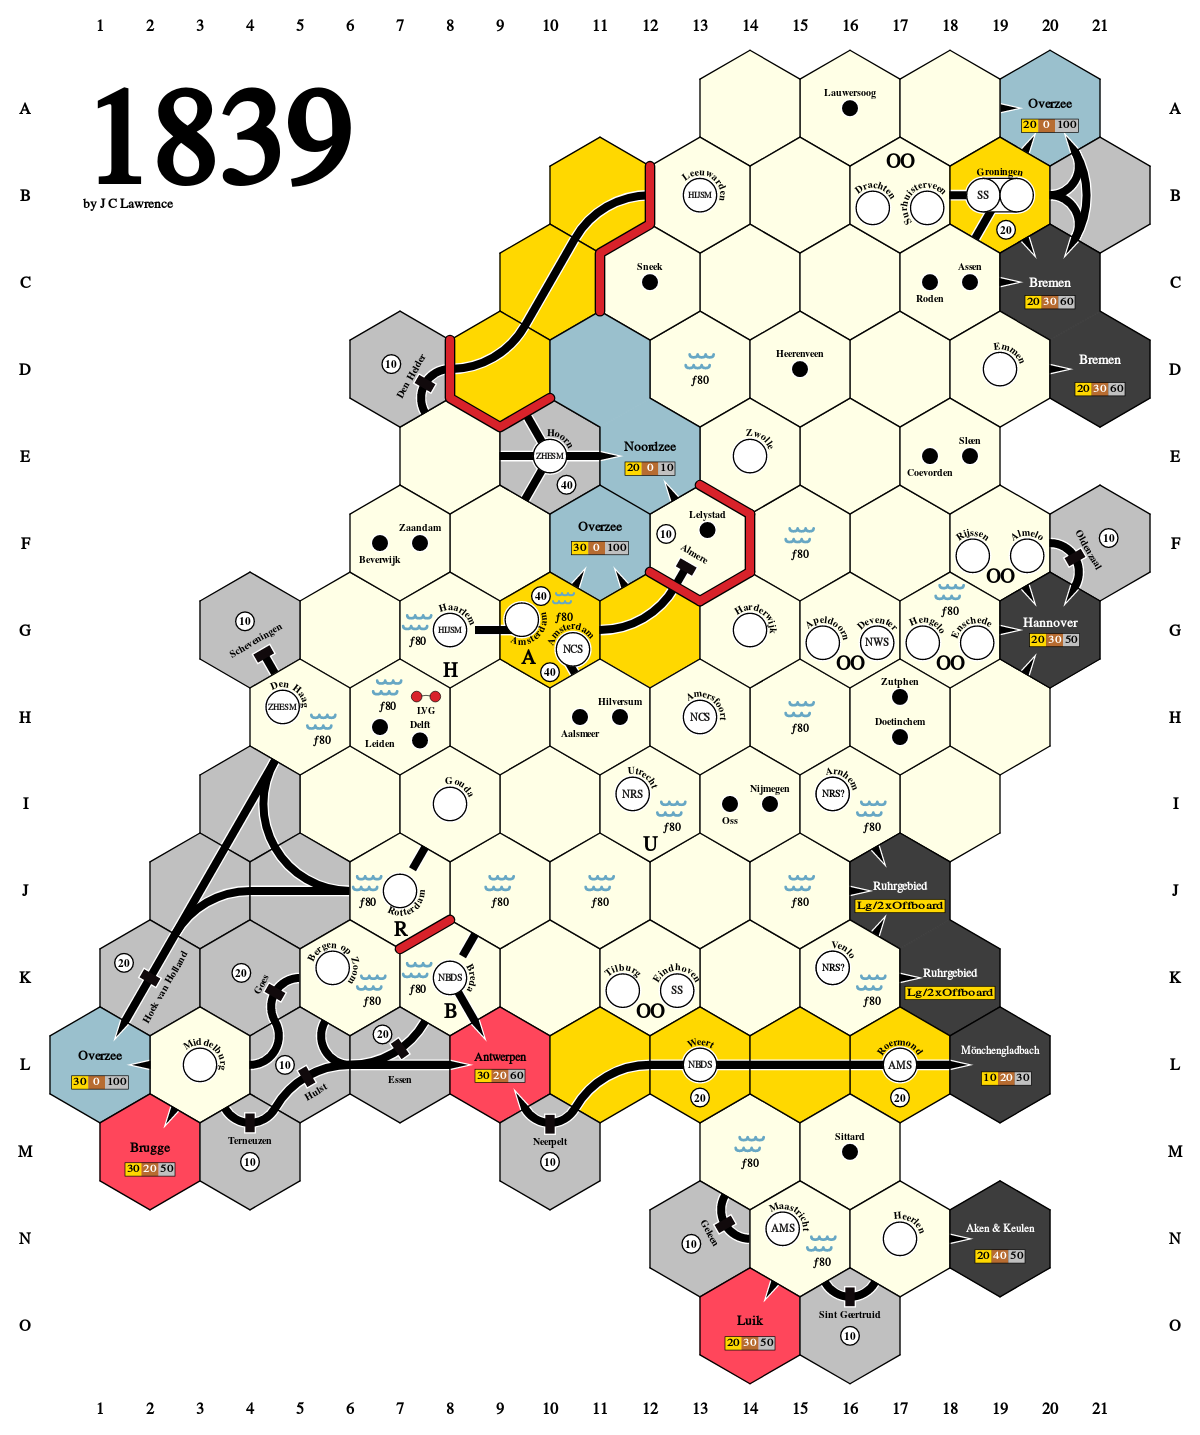
\includegraphics[width=6.75in,height=8.5in]{1839-Map}

\caption{1839 Game Map\label{fig:1828-Game-Map}}
\end{figure*}

\begin{itemize}
\item The map consists of hexagons of various types:
\begin{description}
\item [{Cities:}] City hexagons contain large circles along with the name(s)
of the cities.
\begin{description}
\item [{Big~Cities:}] Are marked with a name (\noun{Amsterdam} (G10),
\noun{Breda} (K8), \noun{Haarlem} (G8), \noun{Rotterdam} (J7), \noun{Utrecht}
(I12)) and have a higher revenue (\emph{some names are abbreviated
for space reasons}).
\item [{OO~City:}] Have two distinct cities on the same tile and are marked
``OO'' but are otherwise the same as a normal city track tile. 
\end{description}
\item [{Towns:}] Town hexagons contain one or two small black circles marking
the towns for hexagons without track, or cross-bars on pre-built track.
\item [{Yellow~hexagons:}] Yellow hexagons represent yellow pre-built
track on the map. They can be upgraded using green track tiles in
light green phase or later (see \secref{Game-Phases} \nameref{sec:Game-Phases}).
\item [{Gray~hexagons:}] Gray hexagons contain pre-built track that may
not be altered nor upgraded. Track tiles cannot be placed on gray
hexagons, nor adjacent to them such that a line of track runs into
a blank gray hexagon-edge.
\item [{Off-board~locations:}] Black (Duitsland/Germany), blue (Overzeesch/Overseas),
and red (Belgie/Belgium) hexagons represent connections to areas not
shown on the map. Black triangles mark separate track connections
to those remote locations. Track tiles may be placed adjacent to them
so that the lines of track connect to the black triangles leading
to the remote connections. Track tiles cannot be placed adjacent to
an off-board hexagon such that a line of track runs into a blank off-board
hexagon-edge.
\item [{Rural~hexagons:}] All other hexagons are rural.
\end{description}
\item Terrain is marked with a wavy line (river) along with the terrain
cost for building track on those hexagons (always \textflorin 80).
\item Revenue centers and off-board locations are marked with their revenue
as a number in a small white circle, or as a series of numbers in
a coloured box matching the game phases at which they start applying
(see \tabref{Game-Phases} \nameref{tab:Game-Phases} \& \subsecref{Run-train(s)}
\nameref{subsec:Run-train(s)}).
\begin{description}
\item [{Exception:}] The revenue value of the Ruhrgebied (J17 \& K18) off-board
is equal to either the largest revenue value on the route, or double
the revenue of the differently coloured off-board at the other end
of the route, whichever is the larger.
\end{description}
\item The hexagon at H7 is marked with a red barbell, denoting that it is
blocked by a private company (see \parref{Het-Laantje-van} \nameref{par:Het-Laantje-van}).
\item Some hexagon edges are blocked by red barriers and track tiles cannot
be placed so as to make a new track connection across that edge before
light red phase (see \parref{track-placement-Overview} \nameref{par:track-placement-Overview}
\& \secref{Game-Phases} \nameref{sec:Game-Phases}).
\item Some hexes are connected by partial track stubs (\noun{Breda} (K8),
\noun{Haarlem} (G8), and \noun{Rotterdam} (J7)). The track stubs on
those hexes constrain future track lays on those hexes to connecting
those edges (see \subsecref{Track-placement-=000026-upgrades} \nameref{subsec:Track-placement-=000026-upgrades})
\item The Bremen (C20 \& D21) and Ruhrgebied (J17 \& K18) off-boards are
each a single location comprised of two hexagons.
\item Related terms:
\begin{description}
\item [{Revenue~center}] A city or town on a hexagon or track tile that
has an income or revenue value. Off-boards are not revenue centers.
\item [{Line~of~track}] A continuous track-connection between a hexagon
edge and a revenue center, or between a specific pair of hexagon edges
on the same or different hexagons.
\end{description}
\end{itemize}

\section{Stock Market\label{sec:Stock-Market}}

\begin{figure}
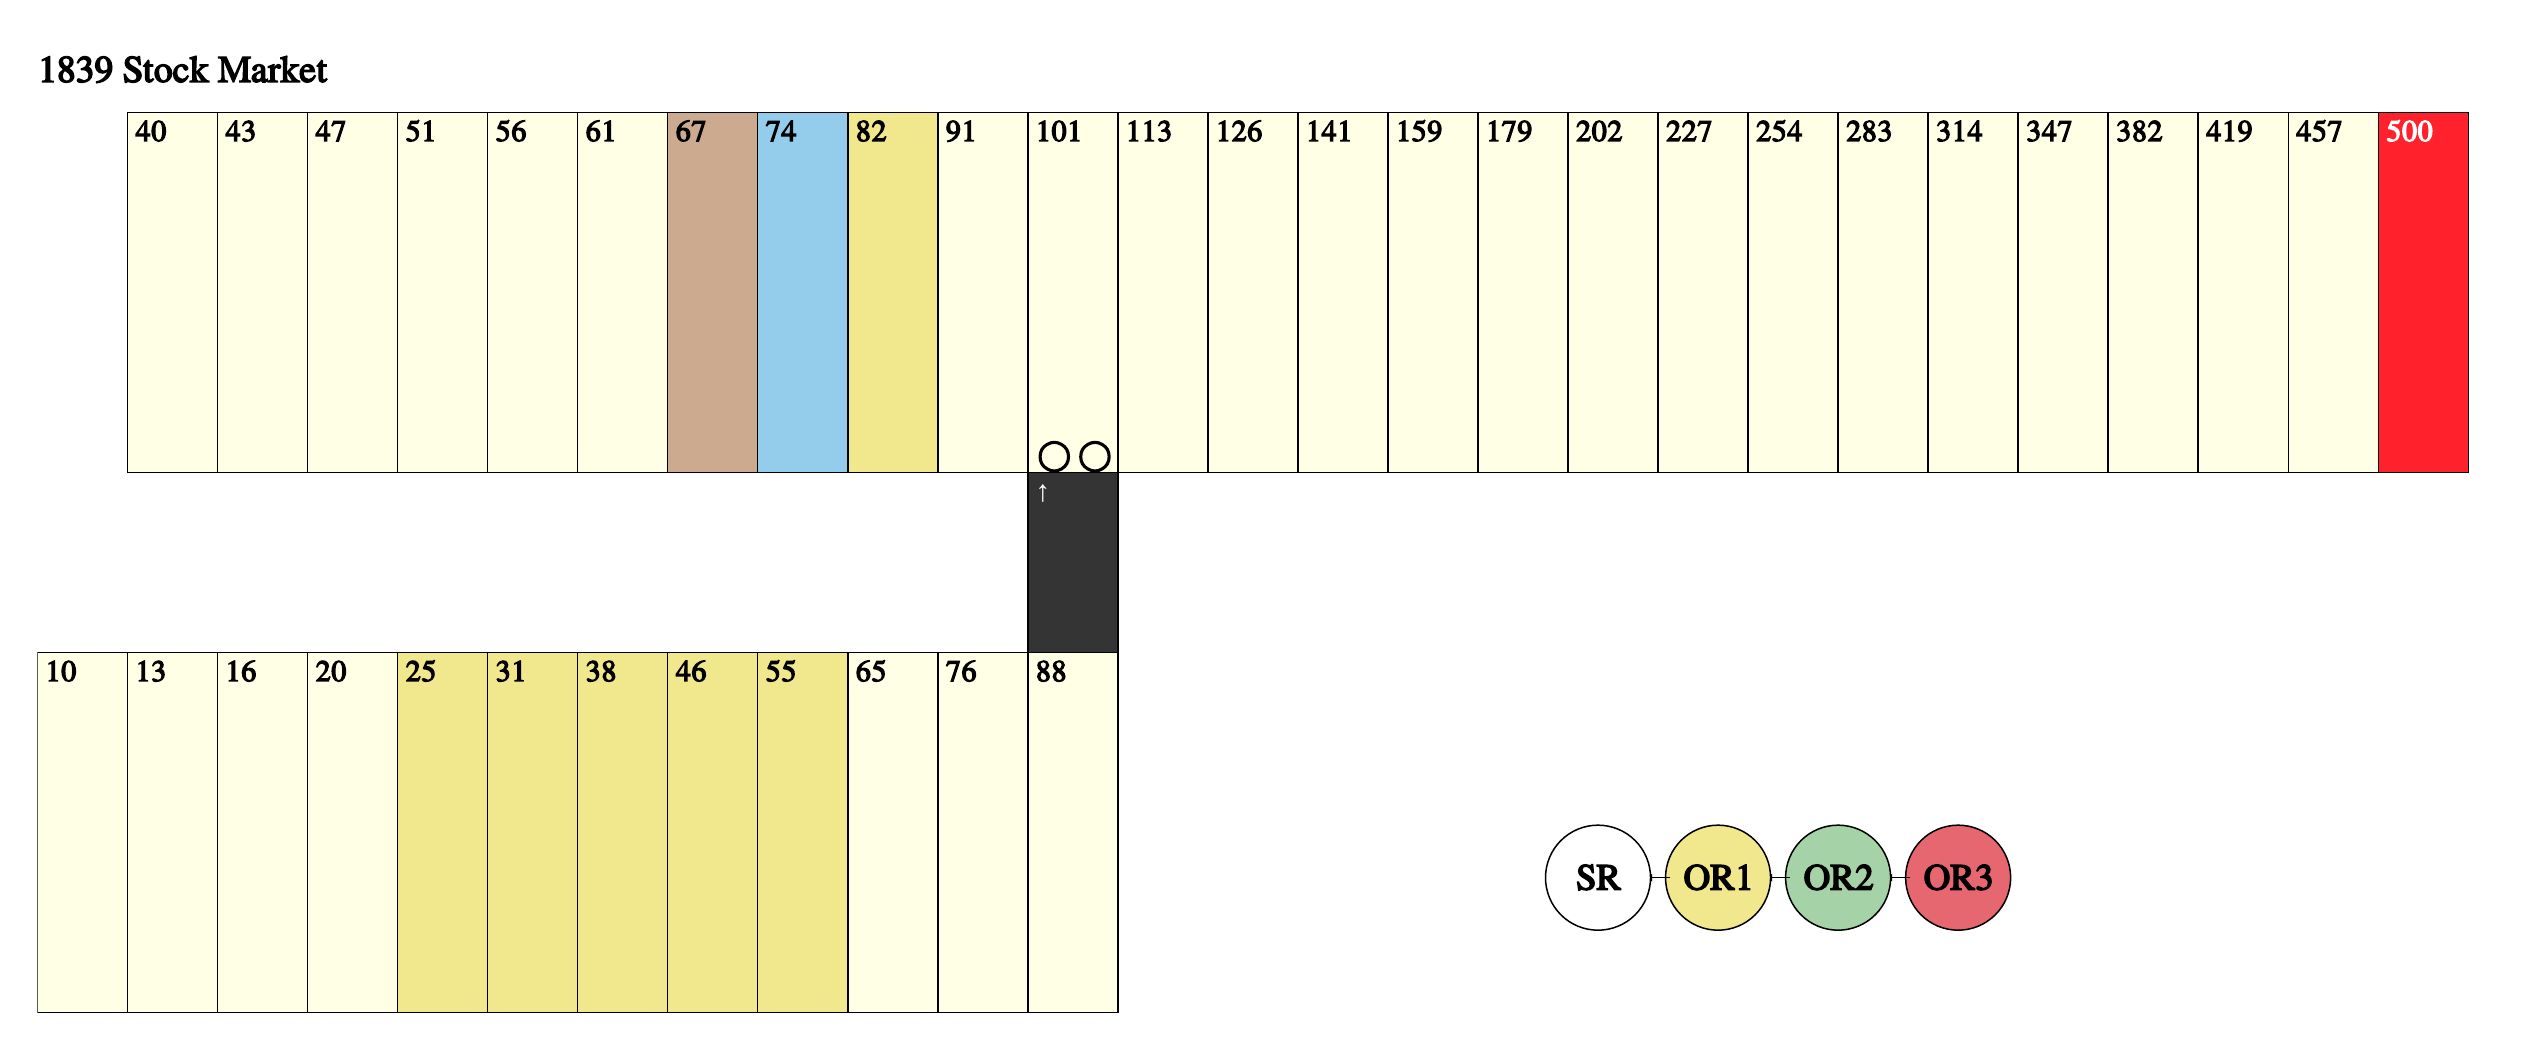
\includegraphics[angle=90,width=1\columnwidth]{1839-Market}

\caption{Stock Market\label{fig:Stock-Market}}
\end{figure}


\subsection{Stock Market overview\label{subsec:Stock-Market-Overview}}
\begin{itemize}
\item Public companies have a stock price that is tracked on the Stock Market
with a stock price marker.
\item The Stock Market consists of two distinct markets:
\begin{itemize}
\item A Local Stock Market with values from \textflorin 10 to \textflorin 65
\item A Major Stock Market with values from \textflorin 40 to \textflorin 300.
\end{itemize}
\item Public Companies with stock prices on the Local Stock Market are Local
Public Companies (see \subsecref{Public-Company-Overview} \nameref{subsec:Public-Company-Overview}).
\item Public Companies with stock prices on the Major Stock Market are Major
Public Companies (see \subsecref{Public-Company-Overview} \nameref{subsec:Public-Company-Overview}).
\item Within each market, potential par prices are marked:
\begin{itemize}
\item When a Public Company is parred, its stock price marker is placed
on the matching location on the Stock Market (see \subsecref{Starting-or-floating}
\nameref{subsec:Starting-or-floating} \& \tabref{Game-Phases} \nameref{tab:Game-Phases}).
\begin{itemize}
\item Lokaalspoorwegen can par at any of the the darker yellow values on
the the Local Stock Market: \textflorin 20, \textflorin 31 or \textflorin 46.
\item Spoorwegmaatschappij can par at (see \secref{Game-Phases} \nameref{sec:Game-Phases}):
\begin{itemize}
\item \textflorin 82 until blue phase.
\item \textflorin 74 until light brown phase.
\item \textflorin 67 in all phases.
\end{itemize}
\item A company cannot par at a price which is the current stock price of
two or more other Public Companies (see \subsecref{Starting-or-floating}
\nameref{subsec:Starting-or-floating}).
\begin{description}
\item [{Exception:}] The Lokaalspoorwegen parred when the yellow and brown
private companies close are always parred at \textflorin 20 (see \parref{Yellow-private-companies}
\nameref{par:Yellow-private-companies} \& \parref{Brown-private-companies}
\nameref{par:Brown-private-companies} ).
\end{description}
\end{itemize}
\end{itemize}
\item Both markets have large areas of pale-background spaces with no special
rules.
\item The \textflorin 300 price on the Major Stock Market has a red background.
The game ends if a stock price marker reaches \textflorin 300 (see
\subsecref{Game-end-criteria} \nameref{subsec:Game-end-criteria}).
\item Public company stock prices and their markers move in well-defined
ways (see \subsecref{Stock-price-movement} \nameref{subsec:Stock-price-movement}).
\end{itemize}

\subsection{Stock price movement\label{subsec:Stock-price-movement}}
\begin{itemize}
\item The current stock price of a Public Company's shares is recorded on
a Stock Market with a stock price marker.
\item Stock price markers can move left or right along that Stock Market.
\begin{itemize}
\item If a stock price is to be moved left when it is already at the left
end of its Stock Market, it isn't moved.
\item The game will end if a stock price marker reaches the largest price
on the Major Stock Market (\textflorin 300) (see \secref{Game-End}
\nameref{sec:Game-End}).
\end{itemize}
\item When a stock price marker is moved, it is placed under any stock price
markers already present in the new location.
\item For each 10\% share sold by a player that isn't immediately redeemed
by that company, the stock price marker is moved left once (see \subsecref{Selling-shares}
\nameref{subsec:Selling-shares} \& \subsecref{Redeeming-shares}
\nameref{subsec:Redeeming-shares}).
\begin{itemize}
\item If shares of multiple companies are sold at the same time, the seller
must decide the order in which they are sold and thus the order in
which their stock price markers are moved (see \subsecref{Selling-shares}
\nameref{subsec:Selling-shares}).
\end{itemize}
\item At the end of each Stock Round, the stock price markers of Public
Companies that have:
\begin{itemize}
\item One or more shares in the Bank Pool are moved left once (see \subsecref{company-operating-order}
\nameref{subsec:company-operating-order}).
\item No shares left in both the IPO and Bank Pool are moved right once
(see \subsecref{company-operating-order} \nameref{subsec:company-operating-order}).
\end{itemize}
\item When a Public Company operates and pays or withholds a dividend, if
the total dividend paid is:
\begin{description}
\item [{Less~than~the~current~stock~price:}] the stock price is moved
left once.
\item [{Zero~because~the~company~didn't~have~a~train:}] it is moved
left another time.
\item [{Equal~to~or~larger~than~the~current~stock~price:}] the
stock price is moved right once.
\item [{Equal~to~or~larger~than~double~the~current~stock~price:}] the
stock price is moved right a second time.
\item [{(\emph{Local~Public~Companies~only}~Equal~to~~larger~than~quadruple~the~current~stock~price:}] the
stock price is moved right a third time.
\end{description}
\item If a stock price reaches \textflorin 300:
\begin{itemize}
\item At the end of a Stock Round because there were no shares left in the
Bank Pool or IPO of that company, the game ends immediately and the
winner is determined (see \subsecref{Scoring} \nameref{subsec:Scoring}).
\item By paying a dividend during an Operating Round and having the stock
price move to \textflorin 300, the game ends at the end of that Operating
Round (see \subsecref{Stock-price-movement} \nameref{subsec:Stock-price-movement}
\& \secref{Game-End} \nameref{sec:Game-End}).
\end{itemize}
\end{itemize}

\section{Companies\label{sec:Companies}}

\subsection{Company types\label{subsec:Company-types}}
\begin{itemize}
\item There are two types of companies: private companies (see \subsecref{Private-Companies}
\nameref{subsec:Private-Companies}) and Public Companies.
\item Private companies are represented by a single private company certificate,
may pay a revenue to their holder at the start of Operating Rounds,
and may grant their owner a special power, behaviour or benefit.
\item Public companies have shares that players may buy and sell at a share
price that's tracked on one of the Stock Markets (see \secref{Stock-Market}
\nameref{sec:Stock-Market}), and can build track, place station markers,
buy private companies and trains, run trains, pay or withhold dividends
(see \secref{Operating-Rounds} \nameref{sec:Operating-Rounds}) and
be nationalised (see \subsecref{Public-company-nationalisation} \nameref{subsec:Public-company-nationalisation}).
\item There are two types of Public Companies before they are parred, and
two types after they are parred:
\begin{itemize}
\item ``\noun{Lokaalspoorwegen}'' and ``\noun{Spoorwegmaatschappij}``
identify company types before they are parred (see \subsecref{Starting-or-floating}
\nameref{subsec:Starting-or-floating}).
\item ``Local Public Company'' and ``Major Public Company'' identify
company types after they are parred based on which stock market currently
contains their stock price marker (see \subsecref{Starting-or-floating}
\nameref{subsec:Starting-or-floating} \& \secref{Stock-Market} \nameref{sec:Stock-Market}).
\end{itemize}
\end{itemize}

\subsection{Private companies\label{subsec:Private-Companies}}

\subsubsection{Private company general rules\label{subsec:Private-Companies-Overview}}
\begin{itemize}
\item Private companies pay their revenue from the bank to their owners
(a player or a Public Company) at the start of each Operating Round
(see \subsecref{Operating-round-General} \nameref{subsec:Operating-round-General})\noun{.}
Private companies do not otherwise ``operate'' and do not lay track,
or buy or run trains.
\begin{description}
\item [{Exception:}] The owner of the \noun{Rotterdamsche Handelsvereeniging},
if in the game, must pay \textflorin 100 to the bank (see \parref{Rotterdamsche-Bank}
\nameref{par:Rotterdamsche-Bank}) at the start of each Operating
Round.
\end{description}
\item (\emph{Light green phase or later}) Public companies may buy green
private companies from players (see \subsecref{Operating-round-actions}
\nameref{subsec:Operating-round-actions}) at any time during the
operation of the buying company (see \subsecref{Saleable-private-companies}
\nameref{subsec:Saleable-private-companies}).
\item (\emph{Blue phase or later}) Public companies may buy blue private
companies from players (see \subsecref{Operating-round-actions} \nameref{subsec:Operating-round-actions})
at any time during the operation of the buying company (see \subsecref{Saleable-private-companies}
\nameref{subsec:Saleable-private-companies}).
\item When a Public Company buys a private company from a player:
\begin{itemize}
\item Both the director of the buying company and the owner of the private
company must agree to the purchase.
\item The purchase price may range from \textflorin 1 to the private company's
face value and is paid from the buying company's treasury to the selling
player.
\item Bought private companies are moved to their owning company's charter
and future revenues from the private company will be paid to the owning
company's treasury.
\item The owning company may use the special power of the private company,
if any, when the owning company is operating from the point of purchase
onward and as long as the private company has not closed. Some private
company powers can only be used during certain steps of their owning
company's operations.
\end{itemize}
\item Yellow, brown and red private companies cannot be bought by Public
Companies (see \parref{Unsaleable-private-companies} \nameref{par:Unsaleable-private-companies}).
\item The \noun{Het Laantje van Van der Gaag} green private company blocks
the H7 hexagon on the map. A track tile cannot be built or upgraded
at that hexagon by a Public Company until the \noun{Het Laantje van
Van der Gaag} green private company has been bought by a Public Company
or closed (see \parref{Het-Laantje-van} \nameref{par:Het-Laantje-van}).
\item Private companies are discarded from the game when they close.
\end{itemize}

\subsubsection{Saleable private companies\label{subsec:Saleable-private-companies}}

\paragraph{Green private companies\label{par:Green-private-companies}}

\subparagraph{\noun{Het Laantje van Van der Gaag\label{par:Het-Laantje-van}}}
\begin{description}
\item [{Nickname:}] ``yellow tile''
\item [{Face~value:}] \textflorin 90
\item [{Revenue:}] \textflorin 10
\item [{Blocks:}] H7
\item [{Closes:}] When power used or the start of gray phase.
\item [{Power:}] The owning Public Company may place an additional yellow
track tile (all terrain costs or upgrade costs must be paid) in addition
to the Public Company's normal track lay for \textflorin 20. There
is no terrain cost if the placed tile is at H7.
\item [{Use:}] Power may be used at any time during the owning Public Company's
track build.
\end{description}

\subparagraph{\noun{Spoorlijn Roosendaal - Vlissingen\label{par:Spoorlijn-Roosendaal--}}}
\begin{description}
\item [{Nickname:}] ``teleport''
\item [{Face~value:}] \textflorin 100
\item [{Revenue:}] \textflorin 10
\item [{Blocks:}] None.
\item [{Closes:}] When power used or the start of gray phase.
\item [{Power:}] At a total cost of \textflorin 80, the owning Public Company
may place or upgrade a track tile at Arnhem (I16) or Venlo (K16) as
their yellow track lay or upgrade respectively and/or may place a
station marker in an empty and unreserved city location, or in replacement
of a government station marker, on that tile instead of their normal
station placement. The track tile placed or upgraded with the private
at Arnhem (I16) or Venlo (K16) does not need to connect to or be part
of one of the owning Public Company\textquoteright s routes.
\item [{Use:}] Power may be used during the owning company's track build
as the owning Public Company's tile lay and/or upgrade and/or station
marker placement in that Operating Round (see \subsecref{Place-station-marker}
\nameref{subsec:Place-station-marker}).
\end{description}

\paragraph{Blue private companies\label{par:Blue-private-companies}}

\subparagraph{\noun{Kabinet-Rochussen\label{par:Kabinet-Rochussen}}}
\begin{description}
\item [{Nickname:}] ``station move''
\item [{Face~value:}] \textflorin 230
\item [{Revenue:}] \textflorin 30 / \textflorin 0 (when owned by a Public
Company)
\item [{Blocks:}] None
\item [{Closes:}] When power used or the start of gray phase.
\item [{Power:}] Owning Public Company may move one of its placed station
markers to a different location on the map for free. The new location
must be a legal station marker placement location for the company
(ignoring cost) before the move. A government station marker is placed
at the prior station marker location (see \subsecref{Government-railway}
\nameref{subsec:Government-railway}). A station-moving company can
include the moved station marker in its new location as one of the
company's station markers on a route in that Operating Round (see
\subsecref{General-Route-definition} \nameref{subsec:General-Route-definition}).
\begin{description}
\item [{Exception:}] A Public Company can move a station marker (see \parref{Swap-station-markers}
\nameref{par:Swap-station-markers}) to a space in a hexagon that
already contains one of the company's station markers. In this case,
the company director must choose which of the two station markers
in the hexagon to return to the company charter and replace with a
government station marker from the supply (see \parref{Swap-station-markers}
\nameref{par:Swap-station-markers} \& \subsecref{Government-railway}
\nameref{subsec:Government-railway}).
\end{description}
\item [{Use:}] Instead of the owning Public Company's station marker placement
in that Operating Round (see \subsecref{Place-station-marker} \nameref{subsec:Place-station-marker}).
\item [{Note:}] In a 2-player game the\noun{ Kabinet-Rochussen} blue private
company is discarded from the game and not used (see \secref{Game-Setup}
\nameref{sec:Game-Setup}).
\end{description}

\subparagraph{\noun{Koninklijke Fabriek van Stoom en andere Werktuigen} \label{par:Koninklijke-Nederlandsche-Fabriek}}
\begin{description}
\item [{Nickname:}] ``money bags''
\item [{Face~value:}] \textflorin 240
\item [{Revenue:}] \textflorin 20 more than it paid in the previous Operating
Round, starting at \textflorin 0 in the first Operating Round of the
game.
\item [{Blocks:}] None.
\item [{Closes:}] At the start of gray phase.
\item [{Power:}] None.
\item [{Use:}] None.
\item [{Note:}] A small charter is provided to ease tracking this private
company's revenue.
\end{description}

\subparagraph{\noun{Diepenbrock en Reigers te Ulft\label{par:Diepenbrock-en-Reigers}}}
\begin{description}
\item [{Nickname:}] ``brown train''
\item [{Face~value:}] \textflorin 250
\item [{Revenue:}] \textflorin 0
\item [{Blocks:}] None
\item [{Closes:}] At the start of dark brown phase.
\item [{Power:}] Converts to a dark brown train at the start of dark brown
phase. (For ease of tracking, the dark brown train is assigned to
the private during setup (see \secref{Game-Setup} \nameref{sec:Game-Setup})
and accompanies the private until it closes) If the private company
is already owned by a Public Company, the train is placed in that
Public Company's treasury. If the private company is owned by a player,
the train is given to the player and may be freely assigned to any
company at any time in dark brown phase or later. If a player owning
the \noun{Diepenbrock en Reigers te Ulft} bankupts or concedes (see
\secref{Player-Bankruptcy}\nameref{sec:Player-Bankruptcy}), then
the matching dark brown train is discarded from the supply. Should
a gray train be purchased while the dark brown train from the \noun{Diepenbrock
en Reigers te Ulft} is held by a player and not assigned to a company,
then it is immediately removed from the game without recompense.
\end{description}

\subparagraph{\noun{Cr�dit Mobilier\label{par:Cr=0000E9dit-Mobilier}}}
\begin{description}
\item [{Nickname:}] ``Cr�dit''
\item [{Face~value:}] \textflorin 260
\item [{Revenue:}] \textflorin 0
\item [{Blocks:}] None
\item [{Closes:}] At the start of dark brown phase.
\item [{Power:}] When closed converts to \textflorin 800 in cash taken
from the bank and the \noun{Rotterdamsche Handelsvereeniging} red
private company, both in the same location as this blue private company
(see \subsecref{Red-private-companies} \nameref{subsec:Red-private-companies}).
\item [{Use:}] None.
\item [{Note:}] If owned by a Public Company when the Public Company is
nationalised (see \subsecref{Public-company-nationalisation} \nameref{subsec:Public-company-nationalisation}),
then the \noun{Rotterdamsche Handelsvereeniging} red private company
is given to the director of the nationalised company (see \subsecref{Red-private-companies}
\nameref{subsec:Red-private-companies} \& \subsecref{Public-company-nationalisation}
\nameref{subsec:Public-company-nationalisation}).
\item [{Note:}] In 2-player and 3-player games the\noun{ Cr�dit Mobilier}
blue private company is discarded from the game and not used (see
\secref{Game-Setup} \nameref{sec:Game-Setup}).
\end{description}

\subparagraph{\noun{Weefgoederenfabrique C.T. Stork \& Co\label{par:Weefgoederenfabrique-C.T.-Stork}}}
\begin{description}
\item [{Nickname:}] ``Shares''
\item [{Face~value:}] \textflorin 260
\item [{Revenue:}] \textflorin 30
\item [{Blocks:}] None.
\item [{Closes:}] At the start of gray phase.
\item [{Power:}] Comes with two 10\% shares of the Public Company associated
with the \noun{Albert Voombergh} brown private company during setup
(see \secref{Game-Setup} \nameref{sec:Game-Setup} \& \parref{Brown-private-companies}
\nameref{par:Brown-private-companies}).
\item [{Use:}] None.
\end{description}

\subsubsection{Unsaleable private companies\label{par:Unsaleable-private-companies}}

\paragraph{Yellow private companies\label{par:Yellow-private-companies}}
\begin{itemize}
\item Each of the yellow private companies has the following attributes:
\begin{description}
\item [{Face~value:}] \textflorin 90 (\noun{Lodewijk Pincoffs}), \textflorin 100
(\noun{J J Beijnes})
\item [{Revenue:}] \textflorin 0
\item [{Blocks:}] None.
\item [{Closes:}] \noun{Lodewijk Pincoffs} closes at the start of dark
yellow phase\noun{. J J Beijnes} closes at the start of dark green
phase.
\item [{Power:}] When closed, the owner of the private company must immediately
par the associated Lokaalspoorwegen (see \subsecref{Starting-or-floating}
\nameref{subsec:Starting-or-floating}) at \textflorin 20. The number
of companies with \textflorin 20 stock prices is not checked. If insufficient
home station locations are available, the Lokaalspoorwegen is not
parred, the shares of the company are returned to the supply, and
the owning player instead receives \textflorin 80 from the bank.
\item [{Use:}] None.
\item [{Note:}] Comes with the 20\% director's certificate and two 10\%
share certificates of the assigned Lokaalspoorwegen (see \secref{Game-Setup}
\nameref{sec:Game-Setup}). The \noun{J J Beijnes} additionally comes
with a 10\% share of the Spoorwegmaatschappij associated with the
\noun{August Borsig} brown private company (see \secref{Game-Setup}
\nameref{sec:Game-Setup}).
\end{description}
\end{itemize}

\paragraph{Brown private companies\label{par:Brown-private-companies}}
\begin{itemize}
\item Each of the brown private companies has the following attributes:
\begin{description}
\item [{Face~value:}] \textflorin 210 (\noun{Cornelis Outshoorn}), \textflorin 220
(\noun{August Borsig}) or \textflorin 260 (\noun{Albert Voombergh}).
\item [{Revenue:}] \textflorin 40 (\textflorin 60 for the \noun{Albert
Voombergh})
\item [{Blocks:}] None.
\item [{Closes:}] At the start of light brown phase or when the assigned
Public Company has acquired a train and finished its Operating Round
steps (see \subsecref{Operating-round-General}\nameref{subsec:Operating-round-General},
\tabref{Game-Phases} \nameref{tab:Game-Phases} \& \secref{Game-Phases}
\nameref{sec:Game-Phases}) or if nationalised when a player bankrupts
or concedes (see \secref{Player-Bankruptcy} \nameref{sec:Player-Bankruptcy}
\& \subsecref{Public-company-nationalisation} \nameref{subsec:Public-company-nationalisation}).
If multiple brown private companies are closed at the same time at
the start of Light Brown phase, then they close in ascending order
of face values.
\item [{Power:}] When closed, the owner of the private company must immediately
a Lokaalspoorwegen (see \subsecref{Starting-or-floating} \nameref{subsec:Starting-or-floating})
at \textflorin 20. The number of companies with \textflorin 20 stock
prices is not checked. If no Lokaalspoorwegen is available or insufficient
home station locations are available, the Lokaalspoorwegen is not
parred, the shares of the company are returned to the supply, and
the owning player instead receives \textflorin 80 from the bank.
\item [{Use:}] None.
\item [{Note:}] Comes with the 20\% director's certificate and a 10\% share
certificate of the assigned Spoorwegmaatschappij (see \secref{Game-Setup}
\nameref{sec:Game-Setup}). The player buying the brown private company
must immediately par the matching Spoorwegmaatschappij to an available
par price on the Major Stock Market (see \secref{Stock-Market} \nameref{sec:Stock-Market}
\& \subsecref{Public-companies} \nameref{subsec:Public-companies})\noun{.}
Each of the par prices of the three Spoorwegmaatschappij associated
with brown private companies must be different. 
\end{description}
\end{itemize}

\paragraph{Red private companies \label{subsec:Red-private-companies}}

\subparagraph{Rotterdamsche Handelsvereeniging\noun{\label{par:Rotterdamsche-Bank}}}
\begin{description}
\item [{Face~value:}] \textflorin 0
\item [{Revenue:}] -\textflorin 100
\item [{Blocks:}] None.
\item [{Closes:}] Never.
\item [{Power:}] None (replaces the \noun{Cr�dit Mobilier} blue private
company when it closes -- see \parref{Cr=0000E9dit-Mobilier} \nameref{par:Cr=0000E9dit-Mobilier}).
\item [{Use:}] None.
\item [{Note:}] At the start of each Operating Round the owner of the \noun{Rotterdamsche
Handelsvereeniging} must pay \textflorin 100 to the bank. Emergency
money raising rules can apply (see \subsecref{Emergency-train-buying}
\nameref{subsec:Emergency-train-buying}).
\end{description}

\subsection{Public companies\label{subsec:Public-companies}}

\subsubsection{Public company overview \label{subsec:Public-Company-Overview}}

\begin{sidewaystable*}
\begin{tabular}{>{\centering}p{5cm}cc>{\centering}p{4cm}>{\centering}p{1cm}>{\centering}p{1cm}c}
Name & Symbol & Type & Home & Par on & Can & \multicolumn{1}{>{\centering}p{1.5cm}}{Stations}\tabularnewline
 &  &  & Stations & Market & Re-float? & (total)\tabularnewline
\hline 
\noun{Aken-Maastrichtsche Spoorweg-Maatschappij} & AMS & Spoorwegmaatschappij & \noun{Roermo}nd (L17),\\
\noun{Maastricht} (N15) & Major & No & 5\tabularnewline
\hline 
\noun{Hollandsche IJzeren Spoorweg-Maatschappij} & HIJSM & Spoorwegmaatschappij & \noun{Leeuwarden} (B13),\\
\noun{Haarlem} (G8) & Major & No & 5\tabularnewline
\hline 
\noun{Maatschappij tot Exploitatie van Staatsspoorwegen} & MSS & Spoorwegmaatschappij & \noun{Groningen} (B19), \noun{Eindhoven} (K12) & Major & No & 5\tabularnewline
\hline 
\noun{Noord-Brabantsch-Duitsche Spoorweg-Maatschappi} & NBDS & Spoorwegmaatschappij & \noun{Breda} (K8),\\
\noun{Weert} (L13) & Major & No & 4\tabularnewline
\hline 
\noun{Nederlandsche Centraal Spoorweg-Maatschappij} & NCS & Spoorwegmaatschappij & \noun{Amsterdam} (G10),\\
\noun{Amersfoort} (H13) & Major & No & 3\tabularnewline
\hline 
\noun{Nederlandsche Rhijnspoorweg-Maatschappij} & NRS & Spoorwegmaatschappij & \noun{Utrech} (I12),\\
choice of \noun{Arnhem} (I16)\\
or \noun{Venlo} (K16) & Major & No & 3\tabularnewline
\hline 
\noun{Nederlandsch-Westfaalsche Spoorweg-Maatschappij} & NWS & Spoorwegmaatschappij & \noun{Deventer} (G16) \& Rijssen (F18) & Major & No & 5\tabularnewline
\hline 
\noun{Zuid-Hollandsche Electrische Spoorweg-Maatschappij} & ZHESM & Spoorwegmaatschappij & \noun{Hoorn} (E10),\\
\noun{Den Haag} (H5) & Major & No & 4\tabularnewline
\hline 
\noun{Lokaalspoorwegen \#1} & L1 & Lokaalspoorwegen & (Director-selected) & Local & Yes & 3\tabularnewline
\hline 
\noun{Lokaalspoorwegen \#2} & L2 & Lokaalspoorwegen & (Director-selected) & Local & Yes & 3\tabularnewline
\hline 
\noun{Lokaalspoorwegen \#3} & L3 & Lokaalspoorwegen & (Director-selected) & Local & Yes & 3\tabularnewline
\hline 
\noun{Lokaalspoorwegen \#4} & L4 & Lokaalspoorwegen & (Director-selected) & Local & Yes & 3\tabularnewline
\hline 
\noun{Lokaalspoorwegen \#5} & L5 & Lokaalspoorwegen & (Director-selected) & Local & Yes & 3\tabularnewline
\hline 
\noun{Lokaalspoorwegen \#6} & L6 & Lokaalspoorwegen & (Director-selected) & Local & Yes & 3\tabularnewline
\hline 
\noun{Lokaalspoorwegen \#7} & L7 & Lokaalspoorwegen & (Director-selected) & Local & Yes & 3\tabularnewline
\hline 
\noun{Lokaalspoorwegen \#8} & L8 & Lokaalspoorwegen & (Director-selected) & Local & Yes & 3\tabularnewline
\hline 
\end{tabular}

\caption{Public companies\label{tab:Public-Companies}}
\end{sidewaystable*}

\begin{itemize}
\item There are sixteen Public Companies (see \tabref{Public-Companies}
\nameref{tab:Public-Companies}) across two types: 
\begin{itemize}
\item Spoorwegmaatschappij\noun{: AMS, HIJSM, MSS, NBDS, NCS, NRS, NWS,
ZHESM.}
\item Lokaalspoorwegen\noun{: Lokaalspoorwegen \#1} through \noun{Lokaalspoorwegen
\#8} (\noun{L1} through \noun{L8).}
\end{itemize}
\item Each Public Company consists of:
\begin{itemize}
\item 9 share certificates:
\begin{itemize}
\item One 20\% director's certificate.
\item Eight 10\% certificates.
\end{itemize}
\item 3, 4 or 5 station markers (see \tabref{Public-Companies} \nameref{tab:Public-Companies})
\item A charter for holding and tracking company assets.
\item A stock price marker.
\end{itemize}
\item Public Companies once parred (see \subsecref{Starting-or-floating}
\nameref{subsec:Starting-or-floating}) have a stock price, tracked
on the stock market with a stock price marker (see \subsecref{Stock-price-movement}
\nameref{subsec:Stock-price-movement}).
\begin{itemize}
\item Local Public Companies have stock prices on the Local Stock Market
(see \secref{Stock-Market} \nameref{sec:Stock-Market}).
\item Major Public Companies have stock prices on the Major Stock Market
(see \secref{Stock-Market} \nameref{sec:Stock-Market}).
\end{itemize}
\item Public companies can:
\begin{itemize}
\item (\emph{Light green phase or later}) Buy green private companies (see
\secref{Game-Phases} \nameref{sec:Game-Phases} \& \subsecref{Private-Companies}
\nameref{subsec:Private-Companies}).
\item (\emph{Blue phase or later}) Buy blue private companies (see \secref{Game-Phases}
\nameref{sec:Game-Phases} \& \subsecref{Private-Companies} \nameref{subsec:Private-Companies}).
\item Use the special powers of any private companies they own (see \subsecref{Private-Companies}
\nameref{subsec:Private-Companies}).
\item Place and upgrade track tiles (see \subsecref{Build-track} \nameref{subsec:Build-track}
\& \subsecref{Track-placement-=000026-upgrades} \nameref{subsec:Track-placement-=000026-upgrades})
\item Place or swap station markers (see \subsecref{Place-station-marker}
\nameref{subsec:Place-station-marker}).
\item Buy trains from the supply and other Public Companies (see \subsecref{Buy-train(s)}
\nameref{subsec:Buy-train(s)} \& \secref{Trains-and-Running-Trains}
\nameref{sec:Trains-and-Running-Trains}).
\item Run trains (see \subsecref{Run-train(s)} \nameref{subsec:Run-train(s)}
\& \secref{Trains-and-Running-Trains} \nameref{sec:Trains-and-Running-Trains}).
\end{itemize}
\item (\emph{Prior to blue phase}) Half-pay or withhold dividends (see \subsecref{Pay-or-withhold}
\nameref{subsec:Pay-or-withhold}).
\item (\emph{Blue phase} \emph{or later}) Pay or withhold dividends (see
\subsecref{Pay-or-withhold} \nameref{subsec:Pay-or-withhold}).
\item Related terms:
\begin{description}
\item [{``Local~Public~Company''~\&~``Major~Public~Company'':}] Identify
company types after they are parred based on which stock market currently
contains their stock price marker (see \subsecref{Starting-or-floating}
\nameref{subsec:Starting-or-floating} \& \secref{Stock-Market} \nameref{sec:Stock-Market}).
\begin{itemize}
\item Local and Major Public Companies are subject to different rules (see
\parref{Major-public-company} \nameref{par:Major-public-company}
\& \parref{Local-public-company} \nameref{par:Local-public-company}).
\item Local Public Companies become Major Public Companies if their stock
price reaches or exceeds \textflorin 101 (see \secref{Stock-Market}
\nameref{sec:Stock-Market} \& \parref{Local-public-company} \nameref{par:Local-public-company}).
\end{itemize}
\item [{``Spoorwegmaatschappij``~\&~``Lokaalspoorwegen'':}] Identify
company types before they are parred (see \subsecref{Starting-or-floating}
\nameref{subsec:Starting-or-floating}). Once parred they become Major
Public Companies and Local Public Companies respectively.
\end{description}
\end{itemize}

\subsubsection{Public company types \label{subsec:Public-company-types}}

\paragraph{Before being parred:}

\subparagraph{Lokaalspoorwegen \label{par:Lokaalsporwegen}}
\begin{itemize}
\item The eight Lokaalspoorwegen (L1...L8):
\begin{itemize}
\item Two are associated with yellow private companies during setup (see
\secref{Game-Setup} \nameref{sec:Game-Setup}).
\item Do not have pre-defined home station locations (see \tabref{Public-Companies}
\nameref{tab:Public-Companies}).
\begin{itemize}
\item Home station hexagons are reserved when the company is parred (see
\subsecref{Starting-or-floating} \nameref{subsec:Starting-or-floating}).
\end{itemize}
\item Must be parred on the Local Stock Market as Local Public Companies
(see \secref{Stock-Market} \nameref{sec:Stock-Market}).
\item Are not discarded from the game if nationalised (see \subsecref{Public-company-nationalisation}
\nameref{subsec:Public-company-nationalisation}) and can be floated
again as new companies in subsequent Stock Rounds (see \subsecref{Starting-or-floating}
\nameref{subsec:Starting-or-floating}).
\end{itemize}
\end{itemize}

\subparagraph{Spoorwegmaatschappij \label{par:Spoorwegmaatschappij}}
\begin{itemize}
\item The eight Spoorwegmaatschappij (see \tabref{Public-Companies} \nameref{tab:Public-Companies}):
\begin{itemize}
\item Some are associated with brown private companies during setup (see
\secref{Game-Setup} \nameref{sec:Game-Setup}).
\item Have pre-defined home station location(s) (see \tabref{Public-Companies}
\nameref{tab:Public-Companies}).
\begin{itemize}
\item The \noun{Nederlandsche Rhijnspoorweg-Maatschappij (NRS)} Public Company
has two home stations, one in \noun{Utrecht} (I12) and one in either
\noun{Arhem} (I16) or \noun{Venlo} (K16) (see \subsecref{Starting-or-floating}
\nameref{subsec:Starting-or-floating} \& \subsecref{Operating-round-actions}
\nameref{subsec:Operating-round-actions}).
\end{itemize}
\item Must be parred on the Major Stock Market as Major Public Companies
(see \secref{Stock-Market} \nameref{sec:Stock-Market}).
\item Have varying numbers of home stations and place-able station markers
depending on the company (see \subsecref{Place-station-marker} \nameref{subsec:Place-station-marker}).
\item Are discarded from the game if nationalised (see \subsecref{Public-company-nationalisation}
\nameref{subsec:Public-company-nationalisation}).
\end{itemize}
\end{itemize}

\paragraph{After being parred:}

\subparagraph{Local Public Company \label{par:Local-public-company}}
\begin{itemize}
\item Buy the next-available train from the supply at no cost (\emph{unless
gray or purple}) when they first operate (see \subsecref{Operating-round-actions}
\nameref{subsec:Operating-round-actions}).
\item Track lays, station placements and train routes are not blocked by
government stations (see \subsecref{Build-track} \nameref{subsec:Build-track},
\subsecref{Place-station-marker} \nameref{subsec:Place-station-marker},
\subsecref{Run-train(s)} \nameref{subsec:Run-train(s)} \& \subsecref{Government-railway}
\nameref{subsec:Government-railway}).
\item Train routes cannot include off-boards (see \subsecref{Run-train(s)}
\nameref{subsec:Run-train(s)} \& \secref{Trains-and-Running-Trains}
\nameref{sec:Trains-and-Running-Trains}).
\end{itemize}

\subparagraph{Major Public Company \label{par:Major-public-company}}
\begin{itemize}
\item Buy the next-available train from the supply at cost (\emph{unless
gray or purple}) when they first operate (see \subsecref{Operating-round-actions}
\nameref{subsec:Operating-round-actions}).
\item Track lays, station placements and train routes are blocked by government
stations (see \subsecref{Government-railway} \nameref{subsec:Government-railway}).
\item Train routes can include off-boards (see \subsecref{Run-train(s)}
\nameref{subsec:Run-train(s)} \& \secref{Trains-and-Running-Trains}
\nameref{sec:Trains-and-Running-Trains}).
\end{itemize}

\subsubsection{Public company directors\label{subsec:Company-directors}}
\begin{itemize}
\item The player that holds the most shares of a Public Company (largest
total percentage) is the director of the company, has the 20\% director's
share of the company and controls all of that company's operations
once it has floated (see \subsecref{Starting-or-floating} \nameref{subsec:Starting-or-floating}).
\item The director's certificate can never be sold, only transferred to
another player. Once a company has floated, there is always a player
that owns the 20\% director's certificate and is the director of the
company until the company is nationalised or the game ends (see \subsecref{Public-company-nationalisation}
\nameref{subsec:Public-company-nationalisation} \& \secref{Game-End}
\nameref{sec:Game-End}).
\item If a player acquires shares such that they own a larger percentage
of the Public Company than the current director, they immediately
become the new company director and exchange company certificates
totaling 20\% of the company for the 20\% director's certificate of
the company, taking control of the company charter and its assets.
\item In order to transfer director control of a company via share sales
(see \subsecref{Selling-shares} \nameref{subsec:Selling-shares}
):
\begin{itemize}
\item Another player must own at least 20\% of the company in order for
the exchange to take place.
\item The director's certificate must be exchanged for certificates of the
player with the most shares of the company after the sale, assigning
control of the Public Company and its charter and assets to that player.
\item The previous director must sell sufficient shares of the Public Company
such that they own fewer shares of the Public Company than the new
director after the sale.
\begin{itemize}
\item In the case of a tie among other players for the most shares after
the sale, the next tied player in rotating player number card order
from the current director becomes the new director.
\end{itemize}
\end{itemize}
\end{itemize}

\subsubsection{Public company nationalisation\label{subsec:Public-company-nationalisation}}

\paragraph{Nationalisation overview\label{subsec:Nationalisation-overview}}
\begin{itemize}
\item When a Public Company acquires the first train of a new rank that
rusts other trains, Public Companies may nationalise after the phase
change has completed (\secref{Game-Phases} \nameref{sec:Game-Phases}).
\item In operating order (see \subsecref{company-operating-order} \nameref{subsec:company-operating-order})
each Public Company that still owns a train, including the company
that acquired the rusting train, may nationalise.
\begin{itemize}
\item A player that holds a brown train from the \noun{Diepenbrock en Reigers
te Ulft} blue private company may assign it to a Public Company in
order for it to immediately qualify for nationalisation (see \parref{Diepenbrock-en-Reigers}
\nameref{par:Diepenbrock-en-Reigers}).
\end{itemize}
\item Players cannot buy the director's certificate of a Public Company
from the IPO if they have nationalised a Public Company in the immediately
preceding set of Operating Rounds (see \subsecref{Operating-round-General}
\nameref{subsec:Operating-round-General} \& \subsecref{Nationalisation-overview}
\nameref{subsec:Nationalisation-overview}).
\end{itemize}

\paragraph{Nationalisation process\label{subsec:Nationalisation-process}}
\begin{enumerate}
\item Any cash in the company treasury is returned to the bank.
\item All shares of the company are returned from the players, company treasury,
Bank Pool, and IPO to the supply without recompense.
\item The company's station makers on the map are replaced by government
station markers (see \subsecref{Government-railway} \nameref{subsec:Government-railway}).
\item The company's station markers and the stock price marker are returned
to the supply.
\item All other assets (trains, private companies) held by the company are
discarded from the game without recompense.
\begin{description}
\item [{Exception:}] If the nationalised Public Company owned the \noun{Rotterdamsche
Handelsvereeniging} red private company, then the \noun{Rotterdamsche
Handelsvereeniging} is given to the director of the company being
nationalised (see \parref{Cr=0000E9dit-Mobilier} \nameref{par:Cr=0000E9dit-Mobilier}
\& \parref{Rotterdamsche-Bank} \nameref{par:Rotterdamsche-Bank}).
\end{description}
\item The Public Company charter is returned to the supply.
\end{enumerate}

\subsection{Government railway\label{subsec:Government-railway}}
\begin{itemize}
\item The Government railway (\noun{Nederlandse Spoorwegen} (NS)) is represented
by a number of station markers.
\item Government station markers replace the station markers of:
\begin{itemize}
\item Nationalised Public Companies (see \subsecref{Nationalisation-process}
\nameref{subsec:Nationalisation-process}).
\item The origin of moved station markers (see \parref{Kabinet-Rochussen}
\nameref{par:Kabinet-Rochussen}).
\item Station markers removed when a company acquires two station markers
in the same hexagon (see \parref{Swap-station-markers} \nameref{par:Swap-station-markers}
\& \parref{Kabinet-Rochussen} \nameref{par:Kabinet-Rochussen}).
\end{itemize}
\item Newly parred Local Public Companies may choose government station
marker locations for their home stations (see \parref{Place-a-station}
\nameref{par:Place-a-station} \& \parref{Swap-station-markers} \nameref{par:Swap-station-markers}
\& \parref{Kabinet-Rochussen} \nameref{par:Kabinet-Rochussen}).
\item When placing a station marker during an Operating Round, Public Companies
may replace government station markers (that aren't reserved for new
company home stations) with their own station marker (see see \parref{Place-a-station}
\nameref{par:Place-a-station} \& \parref{Kabinet-Rochussen} \nameref{par:Kabinet-Rochussen}).
\item Government station markers limit Major Public Company operations in
the same manner as other Public Company station markers and do not
limit Local Public Company operations (see \subsecref{Build-track}
\nameref{subsec:Build-track} \& \subsecref{Place-station-marker}
\nameref{subsec:Place-station-marker} \& \subsecref{Run-train(s)}
\nameref{subsec:Run-train(s)}).
\end{itemize}

\section{Track Tiles\label{sec:Track}}

\subsection{Track tiles overview\label{subsec:Track-Tile-Overview}}
\begin{itemize}
\item There are yellow, green, brown and gray track tiles.
\item Track tiles are limited to those available in the supply.
\item At the beginning of the game only yellow track tiles are available.
\item Yellow track tiles are placed directly on rural and city hexagons
of the map.
\item Green track tiles upgrade/replace yellow track tiles and yellow map
hexagons.
\item Brown track tiles upgrade/replace green track tiles.
\item Gray track tiles upgrade/replace brown track tiles.
\item Upgraded track tiles are returned to the supply for later use.
\end{itemize}

\subsection{Track types\label{subsec:Track-types}}
\begin{itemize}
\item Outside of colour, there are three types of track tiles:
\begin{description}
\item [{City}] Have one or more white circles for station markers and a
revenue value (number in a small white circle). Only city track tiles
can be used on city map hexagons, and they cannot be used on any other
map hexagons.
\begin{description}
\item [{Big~City:}] Are marked with a city name or letter (\noun{``A''
}or \noun{``Amsterdam''} (G10), ``\noun{B}'' or \noun{``Breda''}
(K8), \noun{``H''} or \noun{``Haarlem''} (G8), \noun{``R''}
or \noun{Rotterdam''{}''} (J7), \noun{``U''} or \noun{``Utrecht''}
(I12)) and have a higher revenue. Only matching city track tiles can
be used on those cities and they cannot be used on any other map hexagons.
\item [{OO~City:}] Have two distinct cities on the same tile and are marked
``OO'' and have a higher revenue but are otherwise the same as a
normal city track tile. Only OO city track tiles can be used on hexagons
marked ``OO'', and they cannot be used on any other map hexagons.
\end{description}
\item [{Town:}] Have a small cross-bar marking the town with a line of
track passing through it, and a revenue value (number in a small white
circle). Only town track tiles may be placed on town map hexagons,
and they cannot be used on any other map hexagons. 
\begin{description}
\item [{Double~town:}] Have two distinct track lines, each of which has
a small cross-bar marking the separate towns. Only double town track
tiles may be placed on such map hexagons, and they cannot be used
on any other map hexagons.
\end{description}
\item [{Plain}] Have one to four lines of track without towns or cities,
that directly connect pairs of edges of the hexagon. Plain track tiles
can be used on rural map hexagons, and cannot be used on any other
map hexagons.
\end{description}
\end{itemize}

\subsection{Track placement \& upgrades \label{subsec:Track-placement-=000026-upgrades}}

\subsubsection{Track placement overview \label{par:track-placement-Overview}}
\begin{itemize}
\item Only yellow track tiles are available at the beginning of the game.
Later in the game green, brown and finally gray track tiles become
available (see \tabref{Game-Phases} \nameref{tab:Game-Phases} \&
\subsecref{Upgrading-track} \nameref{subsec:Upgrading-track}).
\item Track tiles can be placed on the towns, cities and rural hexagons
of the map and cannot be placed on off-board hexagons or gray pre-built
hexagons (see \secref{Map-Explanation} \nameref{sec:Map-Explanation}).
\item After placing or upgrading a track tile the placing Public Company
must be able to trace a continuous line of track from one of its station
markers to a line of track on the placed track tile without:
\begin{itemize}
\item Passing through a city with all of station-marker spaces filled with
other Public Company's station markers or (for Major Public Companies
) government station markers (see \subsecref{Government-railway}
\nameref{subsec:Government-railway}).
\item Crossing any hexagon-edge twice.
\end{itemize}
\item Track tiles must not be placed such that a line of track:
\begin{itemize}
\item Already present is not preserved by the new track tile. (Only the
connectivity is important, not the exact shape of the line of track)
\begin{description}
\item [{Note:}] Some hexes are connected by partial track stubs (\noun{Breda}
(K8), \noun{Haarlem} (G8), and \noun{Rotterdam} (J7)). The track stubs
on those hexes constrain future track lays on those hexes to connecting
those edges (see \secref{Map-Explanation} \nameref{sec:Map-Explanation})
\end{description}
\item Runs off the edge of the map (no further hexagons).
\item Runs to the edge of a gray pre-built hexagon that doesn't have pre-printed
track running to it.
\item Runs to the edge of an off-board hexagon that doesn't have a black
triangle/arrow to indicate a continuation for the track.
\item Makes a new track connection across a red barrier before light red
phase (see \secref{Map-Explanation} \nameref{sec:Map-Explanation}).
\end{itemize}
\item A company placing a track tile on a water terrain (\textflorin 80)
hexagon that has not previously contained a track tile must pay the
terrain cost from its treasury to the bank before placing the tile
(see \secref{Map-Explanation} \nameref{sec:Map-Explanation}).
\begin{itemize}
\item Once a track tile of a given type is placed in a hexagon, terrain
costs for the hexagon are not paid again in future tile upgrades.
\begin{description}
\item [{Exception:}] The big cities (\noun{Amsterdam} (G10), \noun{Breda}
(K8), \noun{Haarlem} (G8), \noun{Rotterdam} (J7), \noun{Utrecht} (I12))
have an \textflorin 80 upgrade fee for each upgrade.
\end{description}
\end{itemize}
\item If a company places a yellow track tile on an OO city hexagon which
contains one or more station markers, the company director placing
the track tile has free choice as to which cities to allocate the
station markers on the yellow track tile.
\end{itemize}

\subsubsection{Upgrading track\label{subsec:Upgrading-track}}
\begin{itemize}
\item Starting in light green phase:
\begin{itemize}
\item Public companies may upgrade yellow track tiles and yellow map hexagons
to green track tiles (see \tabref{Game-Phases} \nameref{tab:Game-Phases}).
\end{itemize}
\item Starting in light brown phase:
\begin{itemize}
\item Public companies may also upgrade green track tiles to brown track
tiles (see \tabref{Game-Phases} \nameref{tab:Game-Phases}).
\end{itemize}
\item Starting in gray phase:
\begin{itemize}
\item Public companies may also upgrade brown track tiles to gray track
tiles (see \tabref{Game-Phases} \nameref{tab:Game-Phases}).
\end{itemize}
\item When upgrading a track tile:
\begin{itemize}
\item The type of the track tile cannot be changed.
\item Connections of pairs of hexagon edges by lines of track must be preserved.
\item Connections of city circles to hexagon edges by lines of track must
be preserved.
\begin{itemize}
\item The number of city circles on the track tile may be reduced by a track
tile upgrade if all Public Company station markers and all company
stations reservations on the track tile can be placed in city circles
on the upgraded track tile.
\begin{description}
\item [{Note:}] Government station markers may be discarded and returned
to the supply if there are not enough city circles on the upgraded
track tile for them.
\end{description}
\end{itemize}
\item A Public Company cannot upgrade a track tile it has placed in that
same Operating Round.
\end{itemize}
\item The upgraded track tile is returned to the supply for future use.
\item Once a track tile on a river hexagon is upgraded, the terrain cost
is not paid again (see \secref{Map-Explanation} \nameref{sec:Map-Explanation}).
\begin{description}
\item [{Exception:}] The big cities (\noun{Amsterdam} (G10), \noun{Breda}
(K8), \noun{Haarlem} (G8), \noun{Rotterdam} (J7), \noun{Utrecht} (I12))
have an \textflorin 80 upgrade fee for each upgrade (see \subsecref{Upgrading-track}\nameref{subsec:Upgrading-track}).
\end{description}
\item Station markers are moved to their corresponding locations on the
new tile when upgrading a track tile or hexagon.
\end{itemize}

\section{Trains \& Running Trains\label{sec:Trains-and-Running-Trains}}

\subsection{Trains overview\label{subsec:Trains-Overview}}
\begin{itemize}
\item Public companies run and buy trains during Operating Rounds (see \subsecref{Run-train(s)}
\nameref{subsec:Run-train(s)} and \subsecref{Buy-train(s)} \nameref{subsec:Buy-train(s)}).
\item Public companies run trains on ``routes'' to generate revenue (see
\subsecref{Run-train(s)} \nameref{subsec:Run-train(s)}).
\item Different types of trains have different restrictions for their routes
(see \subsecref{Route-definitions-by-train-type} \nameref{subsec:Route-definitions-by-train-type}).
\item Local Public Companies have different restrictions for their routes
than Major Public Companies (see \subsecref{Public-Company-Overview}
\nameref{subsec:Public-Company-Overview} \& \subsecref{Public-Company-Overview}
\nameref{subsec:Public-Company-Overview}).
\item Cities' and towns' revenues can be counted towards a company's revenue
only once, no matter how many of the company's trains include the
city or town in their route.
\begin{description}
\item [{Exception:}] ``R'' trains can count the revenue of a city or
town toward company revenue that a different train run by the same
company has already counted.
\end{description}
\item (\emph{Major Public Companies only}) Off-board revenues can be counted
for each of the company's train routes that include it.
\item The number of trains a Public Company can own is controlled by the
train limit (see \subsecref{Train-Limit} \nameref{subsec:Train-Limit}).
\item Public companies must own at least one train at the end of their turn
in an Operating Round (see \subsecref{Emergency-train-buying} \nameref{subsec:Emergency-train-buying})
\item Trains are available from the supply in colour order:
\begin{itemize}
\item First yellow, then green, blue, brown, red, gray and finally purple.
\item All the trains of a given colour must be bought or discarded from
the supply before the trains of the next colour are available (see
\tabref{Game-Phases} \nameref{tab:Game-Phases} \& \subsecref{Buy-train(s)}
\nameref{subsec:Buy-train(s)}).
\end{itemize}
\item Trains are bought one at a time with any phase changes occurring before
the company buys any more trains in that Operating Round (see \tabref{Game-Phases}
\nameref{tab:Game-Phases}).
\item The purchase of trains of new types causes phase changes and may change
the train limit (see \tabref{Game-Phases} \nameref{tab:Game-Phases}
\& \subsecref{Train-Limit} \nameref{subsec:Train-Limit}).
\item ``R'' trains are guaranteed to run a route in an Operating Round
at least once (see \subsecref{R-trains} \nameref{subsec:R-trains}
\& \secref{Game-Phases} \nameref{sec:Game-Phases}). When they rust,
those:
\begin{itemize}
\item That have already run a route in an Operating Round are discarded
from the game.
\item That have not yet run a route in an Operating Round are discarded
from the game immediately after they do run a route.
\end{itemize}
\end{itemize}

\subsection{Route definition \label{subsec:General-Route-definition}}
\begin{itemize}
\item A route is a single continuous line of track that:
\begin{itemize}
\item Contains at least two revenue centers (town or city) (see \secref{Map-Explanation}
\nameref{sec:Map-Explanation}).
\item Can begin or end at a town, city or (\emph{Major Public Companies
only}) off-board.
\item Must include a city containing one of the owning Public Company's
station makers.
\item Can pass through a city with an open station marker location.
\item (\emph{Local Public Companies only}) Can pass through an otherwise
blocked city that contains a government station marker location (see
\subsecref{Government-railway} \nameref{subsec:Government-railway}).
\item Can include separate revenue centers on the same hexagon (see \subsecref{Track-types}
\nameref{subsec:Track-types}).
\item Can use multiple entirely separate lines of track on the same tile.
\begin{description}
\item [{Note:}] Plain track tiles such as \#16, \#19, \#20 etc and parts
of \#43, \#44, \#45 \& \#46 etc represent railway bridges and thus
lines of track that do not intersect.
\item [{Note:}] The intersections at the center of plain track tiles such
as \#80, \#81, \#82, \#83, \#544, \#545, and \#546 do not limit the
number of routes or trains which may traverse them.
\end{description}
\item Can enter a city from one direction and exit in any other connected
direction.
\end{itemize}
\item Additionally, a route cannot:
\begin{itemize}
\item Cross the same hexagon-edge more than once.
\item Use the same piece of track on a track tile more than once (no matter
how small the track section may be).
\item Pass through a city that doesn't have an open station marker location
and doesn't contain the Public Company's station marker and (\emph{Local
Public Companies only}) doesn't contain a Government station marker
(see \subsecref{Government-railway} \nameref{subsec:Government-railway}).
\begin{itemize}
\item A Public Company that initiates swapping one of its station markers
during its operations cannot use the swapped station marker in that
Operating Round (see \parref{Swap-station-markers} \nameref{par:Swap-station-markers}).
\end{itemize}
\item Run to or through the same revenue center more than once.
\item Have both ends of the route in an off-board of the same colour (black,
blue or red, see \secref{Map-Explanation} \nameref{sec:Map-Explanation}).
\item Cross a red barrier before light red phase (see \secref{Map-Explanation}
\nameref{sec:Map-Explanation} \& \secref{Game-Phases} \nameref{sec:Game-Phases}).
\end{itemize}
\item The routes of multiple trains run by the same Public Company during
an Operating Round cannot share or re-use any line of track.
\begin{itemize}
\item The routes can meet or cross provided that they use entirely separate
sections of track.
\end{itemize}
\item Off-board triangle connections are termini. Routes may not run into
an off-board location via one black triangle and proceed back onto
the board via another (see \secref{Map-Explanation} \nameref{sec:Map-Explanation}).
\item Local Public Companies cannot include off-boards in their routes (see
\parref{Local-public-company} \nameref{par:Local-public-company})
\item (\emph{Major Public Companies only}) The revenue value of the \noun{Ruhrgebied}
(J17 \& K18) off-board is equal to either the largest revenue value
on the route, or double the revenue of the off-board at the other
end of the route, whichever is the larger (see \parref{Major-public-company}
\nameref{par:Major-public-company}).
\end{itemize}

\subsection{Running trains by train-type \label{subsec:Route-definitions-by-train-type}}

\subsubsection{Train types\label{subsec:Train-types}}

\paragraph{\emph{N}~trains \label{subsec:Ntrains}}
\begin{itemize}
\item The route for an \emph{N} train (where \emph{N} is 2 or 4 ) cannot
contain more than a total of \emph{N} revenue centers.
\begin{description}
\item [{Revenue:}] The sum of all the revenue centers on the route whose
revenues are not included in the routes of other non-''R'' trains
(see \subsecref{R-trains} \nameref{subsec:R-trains}) owned by the
company plus (\emph{Major Public Companies only}, see \subsecref{Public-companies}
\nameref{subsec:Public-companies}) any off-boards of different colours
at the ends of the route.
\end{description}
\end{itemize}

\paragraph{N+ trains \label{subsec:N+-trains}}
\begin{itemize}
\item The route for a N+ train (where \emph{N} is 2, 3 or 5) cannot contain
more than a total of N cities. There may be any number of towns on
the route; before, between and after any other revenue centers on
the route.
\begin{description}
\item [{Revenue:}] The sum of all the revenue centers on the route whose
revenues are not included in the routes of other non-''R'' trains
(see \subsecref{R-trains} \nameref{subsec:R-trains}) owned by the
company plus (\emph{Major Public Companies only}, see \subsecref{Public-companies}
\nameref{subsec:Public-companies}) any off-boards of different colours
at the ends of the route.
\end{description}
\end{itemize}

\subsubsection{Train modifiers \label{subsec:Train-modifiers}}

\paragraph{``P'' trains\label{subsec:P-trains}}
\begin{itemize}
\item ``P'' trains can include only one off-board in their route (if owned
by a Major Public Company, see \subsecref{Public-companies} \nameref{subsec:Public-companies}).
\end{itemize}

\paragraph{``R'' trains\label{subsec:R-trains}}
\begin{itemize}
\item ``R'' trains:
\begin{itemize}
\item Can count cities and towns on their routes for revenue that other
trains in the same company have already included for revenue in their
routes.
\item ``R'' trains are guaranteed to run a route in an Operating Round
at least once (see \secref{Game-Phases} \nameref{sec:Game-Phases}).
When they rust, those:
\begin{itemize}
\item That have already run a route in an Operating Round are discarded
from the game.
\item That have not yet run a route in an Operating Round are discarded
from the game immediately after they do run a route.
\end{itemize}
\item An ``R'' train owned by a company during the Run Train(s) portion
of the company's operations, and which contributed revenue to the
company's income is considered to have run a route in that Operating
Round (see \subsecref{Run-train(s)} \nameref{subsec:Run-train(s)}).
\begin{description}
\item [{Note:}] \emph{``R'' trains that have not yet run a route can
be marked by placing them sideways on company charters, turning them
vertical as they run a route. Non-''R'' trains can then also be
kept vertical on their company charters by default, thus having all
vertical trains on charters being immediately subject to rusting.}
\end{description}
\end{itemize}
\end{itemize}

\subsection{Train limit\label{subsec:Train-Limit}}
\begin{itemize}
\item The number of trains a Public Company can own is limited by the game
phase (see \subsecref{Buy-train(s)} \nameref{subsec:Buy-train(s)}
\& \secref{Game-Phases} \nameref{sec:Game-Phases}). A Public Company
can own trains up to the current train limit.
\item A Public Company that has not reached its train limit may buy trains
that would cause it to exceed the train limit after the game phase
change caused by the purchase takes effect.
\item Train limits are checked and enforced on all Public Companies as each
train is bought.
\begin{itemize}
\item A Public Company with more trains than the current train limit must
discard its trains (director's choice) from the game until it is within
the current train limit.
\end{itemize}
\end{itemize}

\section{Game Phases \label{sec:Game-Phases}}

\subsection{Light yellow phase}
\begin{itemize}
\item The game begins in light yellow phase.
\item Yellow track tiles are available.
\item Light yellow trains are available.
\item Red barriers between map hexagons block station lays, train routes
and some track builds.
\item Off-boards with multiple revenue values use the first (yellow) value.
\item Other Public Companies cannot buy the last train in a Local Public
Company.
\item Local Public Companies may only pay half-dividends or withhold dividends.
\item Train limit is 3.
\item There is 1 Operating Round per set after Stock Rounds.
\end{itemize}

\subsection{Dark yellow phase}
\begin{itemize}
\item Yellow track tiles are available.
\item Dark yellow trains are available.
\item Red barriers between map hexagons block station lays, train routes
and some track builds.
\item Off-boards with multiple revenue values use the first (yellow) value.
\item Other Public Companies cannot buy the last train in a Local Public
Company.
\item Local Public Companies may only pay half-dividends or withhold dividends.
\item Train limit is 3.
\item There is 1 Operating Round per set after Stock Rounds.
\end{itemize}

\subsection{Light green phase}
\begin{itemize}
\item Light green phase starts with the purchase of the first light green
train.
\item Green private companies may be bought by Public Companies.
\item Green and yellow track tiles are available.
\item Red barriers between map hexagons block station lays, train routes
and some track builds.
\item Off-boards with multiple revenue values use the first (yellow) value.
\item Other Public Companies cannot buy the last train in a Local Public
Company.
\item Local Public Companies may only pay half-dividends or withhold dividends.
\item Train limit is 3.
\item There are 2 Operating Rounds per set after Stock Rounds.
\end{itemize}

\subsection{Dark green phase}
\begin{itemize}
\item Dark green phase starts with the purchase of the first dark green
train.
\item Green private companies may be bought by Public Companies.
\item Green and yellow track tiles are available.
\item Red barriers between map hexagons block station lays, train routes
and some track builds.
\item Off-boards with multiple revenue values use the first (yellow) value.
\item All light yellow trains are discarded from the game.
\item Companies with a dark yellow, light green or or dark green train can
nationalise at the start of dark green phase.
\item Other Public Companies cannot buy the last train in a Local Public
Company.
\item Local Public Companies may only pay half-dividends or withhold dividends.
\item Train limit is 3.
\item There are 2 Operating Rounds per set after Stock Rounds.
\end{itemize}

\subsection{Blue phase}
\begin{itemize}
\item Blue phase starts with the purchase of the first blue train.
\item Green and blue private companies may be bought by Public Companies.
\item Green and yellow track tiles are available.
\item Red barriers between map hexagons block station lays, train routes
and some track builds.
\item Off-boards with multiple revenue values use the first (yellow) value.
\item All dark yellow trains are discarded from the game.
\item Companies with a light green, dark green or blue train can nationalise
at the start of blue phase.
\item Other Public Companies can buy the last train in a Local Public Company.
\item Local Public Companies may only pay or withhold dividends.
\item Train limit is 3.
\item There are 2 Operating Rounds per set after Stock Rounds.
\end{itemize}

\subsection{Light brown phase}
\begin{itemize}
\item Light brown phase starts with the purchase of the first light brown
train.
\item Green and blue private companies may be bought by Public Companies.
\item All remaining Brown private companies close.
\item Brown, green and yellow track tiles are available.
\item Red barriers between map hexagons block station lays, train routes
and some track builds.
\item Off-boards with multiple revenue values use the second (brown) value.
\item All light green trains are discarded from the game.
\item Companies with a dark green, blue or light brown train can nationalise
at the start of light brown phase.
\item Other Public Companies can buy the last train in a Local Public Company.
\item Local Public Companies may only pay or withhold dividends.
\item Train limit is 3.
\item There are 2 Operating Rounds per set after Stock Rounds.
\end{itemize}

\subsection{Medium brown phase}
\begin{itemize}
\item Medium brown phase starts with the purchase of the first medium brown
train.
\item Green and blue private companies may be bought by Public Companies.
\item Brown, green and yellow track tiles are available.
\item Red barriers between map hexagons block station lays, train routes
and some track builds.
\item Off-boards with multiple revenue values use the second (brown) value.
\item All dark green trains are discarded from the game.
\item Companies with a blue, light brown or medium brown train can nationalise
at the start of medium brown phase.
\item Other Public Companies can buy the last train in a Local Public Company.
\item Local Public Companies may only pay or withhold dividends.
\item Train limit is 3.
\item There are 2 Operating Rounds per set after Stock Rounds.
\end{itemize}

\subsection{Dark brown phase}
\begin{itemize}
\item Dark brown phase starts with the purchase of the first dark brown
train.
\item Green and blue private companies may be bought by Public Companies.
\item The \noun{Diepenbrock en Reigers te Ulft} blue private company converts
to a dark brown train.
\item The \noun{Cr�dit Mobilier} blue private company converts to \textflorin 740
and the red \noun{Rotterdamsche Handelsvereeniging} private company.
\item Brown, green and yellow track tiles are available.
\item Red barriers between map hexagons block station lays, train routes
and some track builds.
\item Off-boards with multiple revenue values use the second (brown) value.
\item All blue trains are discarded from the game.
\item Companies with a light brown, medium brown, or dark brown train can
nationalise at the start of dark brown phase.
\item Other Public Companies can buy the last train in a Local Public Company.
\item Local Public Companies may only pay or withhold dividends.
\item Train limit is 3.
\item There are 2 Operating Rounds per set after Stock Rounds.
\end{itemize}

\subsection{Light red phase}
\begin{itemize}
\item Light red phase starts with the purchase of the first light red train.
\item Brown, green and yellow track tiles are available.
\item Red barriers between map hexagons don't block track builds, station
lays or train routes.
\item Off-boards with multiple revenue values use the second (brown) value.
\item All light brown trains that have operated and run a route are discarded
from the game.
\item Any remaining light brown trains are discarded immediately after the
next time they operate and run a route.
\item Companies with a medium brown, dark brown or light red train can nationalise
at the start of light red phase.
\item Other Public Companies can buy the last train in a Local Public Company.
\item Local Public Companies may only pay or withhold dividends.
\item Train limit is 2.
\item There are 3 Operating Rounds per set after Stock Rounds.
\end{itemize}

\subsection{Dark red phase}
\begin{itemize}
\item Dark red phase starts with the purchase of the first dark red train.
\item Brown, green and yellow track tiles are available.
\item Red barriers between map hexagons don't block track builds, station
lays or train routes.
\item Off-boards with multiple revenue values use the second (brown) value.
\item All medium brown trains that have operated and run a route are discarded
from the game.
\item Any remaining medium brown trains are discarded immediately after
the next time they operate and run a route.
\item Companies with a dark brown, light red or dark red train can nationalise
at the start of dark red phase.
\item Other Public Companies can buy the last train in a Local Public Company.
\item Local Public Companies may only pay or withhold dividends.
\item Train limit is 2.
\item There are 3 Operating Rounds per set after Stock Rounds.
\end{itemize}

\subsection{Gray phase}
\begin{itemize}
\item Gray phase starts with the purchase of the first gray train.
\item All remaining private companies close other than the \noun{Rotterdamsche
Handelsvereeniging} close (see \parref{Rotterdamsche-Bank} \nameref{par:Rotterdamsche-Bank})
\item Gray, brown, green and yellow track tiles are available.
\item Red barriers between map hexagons don't block track builds, station
lays or train routes.
\item Off-boards with multiple revenue values use the third (gray) value.
\item All dark brown trains that have operated and run a route are discarded
from the game.
\item Any remaining dark brown trains are discarded immediately after the
next time they operate and run a route.
\item Companies with a R-type train (that hasn't yet run), or a red or gray
train can nationalise at the start of gray phase.
\item Other Public Companies can buy the last train in a Local Public Company.
\item Local Public Companies may only pay or withhold dividends.
\item Train limit is 2.
\item There are 3 Operating Rounds per set after Stock Rounds.
\end{itemize}

\subsection{Purple phase}
\begin{itemize}
\item Purple phase starts with the purchase of the first purple train.
\item Gray, brown, green and yellow track tiles are available.
\item Red barriers between map hexagons don't block track builds, station
lays or train routes.
\item Off-boards with multiple revenue values use the third (gray) value.
\item All light red and dark red trains that have operated and run a route
are discarded from the game.
\item Any remaining light red or dark red trains are discarded immediately
after the next time they operate and run a route.
\item Companies with an R-type train (that hasn't yet run) or a gray train
can nationalise at the start of purple phase.
\item Other Public Companies can buy the last train in a Local Public Company.
\item Local Public Companies may only pay or withhold dividends.
\item Train limit is 2.
\item There are 3 Operating Rounds per set after the Stock Round.
\item The game ends after the first set of Operating Rounds in purple phase.
\end{itemize}

\end{document}
